% !TeX root = thesis.tex
\gdef\mainthesisfile{}
% !TeX root = thesis.tex
\ifdefined\UtilIncluded
  \renewcommand{\startchapter}[1]{}
  \renewcommand{\stopchapter}{}
\else

\newcommand{\startchapter}[1]{\begin{document}\setcounter{chapter}{#1}\addtocounter{chapter}{-1}}
\newcommand{\stopchapter}{\end{document}}


\documentclass[a4paper]{book}
\usepackage[utf8]{inputenc}

\usepackage{amsfonts,amsmath, amsthm, amssymb}
\usepackage{xspace}
\usepackage[hidelinks,bookmarks,pdfusetitle]{hyperref}
\usepackage{listings}
\usepackage[pdftex]{graphicx}
\usepackage{bm}
\usepackage[english]{babel}
\usepackage{caption}
\usepackage{subcaption}
\usepackage[usenames,dvipsnames]{xcolor}
\usepackage{physics}
\usepackage{multicol}
\usepackage{xstring}
\usepackage{pythonhighlight}
\usepackage{parskip}
\usepackage{thmtools}
\usepackage{relsize}
\usepackage{bookmark}
\usepackage{lmodern}
\usepackage{ifthen}
\usepackage{biblatex}
\usepackage{csquotes}

\addbibresource{references.bib}

\newtheorem{theorem}{Theorem}
\newtheorem{lemma}[theorem]{Lemma}
\newtheorem{corollary}[theorem]{Corollary}

\DeclareRobustCommand{\oneD}{{1{\relsize{-1}D}}\xspace}
\DeclareRobustCommand{\twoD}{{2{\relsize{-1}D}}\xspace}
\DeclareRobustCommand{\threeD}{{3{\relsize{-1}D}}\xspace}
\DeclareRobustCommand{\cpp}{{{C\nolinebreak[4]\hspace{-.05em}\raisebox{.4ex}{\relsize{-3}\textbf{++}}}\xspace}}
\pdfstringdefDisableCommands{%
    \def\cpp{C++}%
    \def\oneD{1D}%
    \def\twoD{2D}%
    \def\threeD{3D}%
}

\newcommand{\longchapter}[2][]{%
    \chapter[#2]{#2}%
    \ifthenelse{\equal{#1}{}}{}{\chaptermark{#1}}}

\fi
\gdef\UtilIncluded{}



\title{Algorithms for time-independent Schrödinger equations}
\author{Toon Baeyens}

\begin{document}

% !TeX root = thesis.tex
\newgeometry{right=40mm, bottom=10mm}
\begin{titlepage}
    \AddToShipoutPicture*{
        \put(0,0){%
            \parbox[b][\paperheight]{\paperwidth}{%
                \hfill\scalebox{-1}[1]{
\includegraphics[width=\paperheight,height=4cm,angle=90]{img/titlepage/background_clean.pdf}}\hspace{5mm}
            }}}


    \begin{minipage}{6cm}
        \begin{flushleft}
            \relsize{-1}
            Department of Applied Mathematics, \\
            Computer Science and Statistics

            \vspace{3mm}

            {\relsize{+1}Faculty of Sciences}
        \end{flushleft}
    \end{minipage}

    \vspace{4cm}

    \begin{center}
        {\fontfamily{qag}\selectfont
        \textbf{\relsize{+3} Algorithms for time-independent\\Schrödinger equations}
        }

        % \vspace{0.5cm}
        % Constant perturbation method

        \vspace{5mm}

        \textbf{\relsize{+1} Toon Baeyens}

    \end{center}

    \vspace{1cm}

    \begin{flushleft}
        Supervisors \\
        prof. dr. Marnix Van Daele\\
        prof. dr. Joris Van der Jeugt
    \end{flushleft}

    \vfill

    \begin{center}
        Dissertation submitted in partial fulfillment\\
        of the requirements for the degree of \\
        Doctor of Science: Mathematics

        \vspace{5mm}

        April 2023
    \end{center}

    \vspace{5mm}

    \begin{minipage}{5cm}
        \hspace{-1cm}\includegraphics[width=5cm]{img/logo_ugent.pdf}
    \end{minipage}%
    \hfill%

\end{titlepage}
\restoregeometry


\chapter*{Table of contents}
\addcontentsline{toc}{chapter}{Table of contents}
\markboth{Table of contents}{Table of contents}
\makeatletter
\@starttoc{toc}
\makeatother

% !TeX root = chapter_preface.tex
% !TeX root = thesis.tex
\ifdefined\UtilIncluded
  \renewcommand{\startchapter}[1]{}
  \renewcommand{\stopchapter}{}
\else

\newcommand{\startchapter}[1]{\begin{document}\setcounter{chapter}{#1}\addtocounter{chapter}{-1}}
\newcommand{\stopchapter}{\end{document}}


\documentclass[a4paper]{book}
\usepackage[utf8]{inputenc}

\usepackage{amsfonts,amsmath, amsthm, amssymb}
\usepackage{xspace}
\usepackage[hidelinks,bookmarks,pdfusetitle]{hyperref}
\usepackage{listings}
\usepackage[pdftex]{graphicx}
\usepackage{bm}
\usepackage[english]{babel}
\usepackage{caption}
\usepackage{subcaption}
\usepackage[usenames,dvipsnames]{xcolor}
\usepackage{physics}
\usepackage{multicol}
\usepackage{xstring}
\usepackage{pythonhighlight}
\usepackage{parskip}
\usepackage{thmtools}
\usepackage{relsize}
\usepackage{bookmark}
\usepackage{lmodern}
\usepackage{ifthen}
\usepackage{biblatex}
\usepackage{csquotes}

\addbibresource{references.bib}

\newtheorem{theorem}{Theorem}
\newtheorem{lemma}[theorem]{Lemma}
\newtheorem{corollary}[theorem]{Corollary}

\DeclareRobustCommand{\oneD}{{1{\relsize{-1}D}}\xspace}
\DeclareRobustCommand{\twoD}{{2{\relsize{-1}D}}\xspace}
\DeclareRobustCommand{\threeD}{{3{\relsize{-1}D}}\xspace}
\DeclareRobustCommand{\cpp}{{{C\nolinebreak[4]\hspace{-.05em}\raisebox{.4ex}{\relsize{-3}\textbf{++}}}\xspace}}
\pdfstringdefDisableCommands{%
    \def\cpp{C++}%
    \def\oneD{1D}%
    \def\twoD{2D}%
    \def\threeD{3D}%
}

\newcommand{\longchapter}[2][]{%
    \chapter[#2]{#2}%
    \ifthenelse{\equal{#1}{}}{}{\chaptermark{#1}}}

\fi
\gdef\UtilIncluded{}


\startchapter{0}

\undefinedlabel{cha:c1}{1}
\undefinedlabel{cha:c2}{2}
\undefinedlabel{cha:c3}{3}
\undefinedlabel{cha:c4}{4}

\chapter*{Preface}
\addcontentsline{toc}{chapter}{Preface}

A thesis is a work of long breath\footnote{This is a literal translation of the Dutch expression: `\foreignlanguage{dutch}{Een werk van lange adem}'.}. In the past five years, I have worked on this project. In this book you can find my process in learning about and contributing to the numerical study of Schrödinger equations.

This thesis is written from quite a technical perspective and is definitely not suited as an introductory text to the subject. Following along will require quite a lot of background knowledge. The text assumes you are already familiar with (partial) differential equations, numerical methods for solving these and the intricacies when implementing them. So, if you want to know \emph{all} advances written in this work, then trying to read the book cover to cover may be the best way. I tried to logically structure the work with sufficient cross-references and citation.

If however you are still interested in reading this book without a deep technical knowledge, then I recommend skipping the more technical discussions. Starting with the summary will provide you with a basic overview about what you can expect from this work. Chapter~\ref{cha:c1} gives some historical context about mathematical evolution and in particular about the conception of differential equations. Chapters~\ref{cha:c2},~\ref{cha:c3} and~\ref{cha:c4} contain the innovations from this thesis. Each of these chapters starts with some historical background and mathematical motivation, and ends with some numerical experiments to evaluate the performance (both in accuracy as efficiency) of our methods. For simply a cursory examination of my research, these sections may be sufficient.

If still, you are interested in this thesis, however not so much in the mathematics, even then I can provide some guidance on how to read it. I assume you are more interested in doing research in general or even in me personally. In this case you may\footnote{Of course, as the owner of a book you can read it however you want (or even burn it). So, not that you need it, but you definitely have my permission to skip (large) parts, if they are not of interest to you.} just skip chapters~\ref{cha:c2},~\ref{cha:c3} and~\ref{cha:c4} entirely. The summary and chapter~\ref{cha:c1} may provide sufficient context. For some personal notes, I recommend taking a look at the closing remarks at the end of this work as well.

In the introductory paragraph I stated that this research came into fruition within the past five years. In the most literal sense, this is of course true. Practically however, doing research is quite an individual pursuit, and as such it is quite a personal one. Each researcher is different and experiences the world around them uniquely. This difference, in part, relies on the background of the (mathematical) education of the researcher. In my case, I think I can say that my `mathematical career' started a good fifteen years ago. My interest in and passion for mathematics become abundantly clear\footnote{To the detriment of the non-science courses.} throughout high school. My mathematical adventure really took off when I started at Ghent University, now, ten years later, I can close this chapter with the completion of a PhD in mathematics.


\section*{Acknowledgement}
\addcontentsline{toc}{section}{Acknowledgement}

Even though doing research is quite a lonely process, I was never alone. There are many people who let me find myself and help grow me grow. Here I want to seize the opportunity to thank them wholeheartedly.

% First and foremost my very best friend...

% Marnix (and also Joris)

% parents and family

% Ward (For helping me write)

% Friends and colleages. Many friends became colleages, and many colleages became friends.
% Enumerate Wouter, Frederik, Sam, David, Bart, Jorn
% Enumerate Dieter, Annick, Adnan, Niko, Robbert, Heidi, Rien, Asmus, Roy, ... (Wie nog?)
%            Koffiepauzes: Kris, Nico,
%            Steven, Alexis (Nagelezen!), Charlotte
% Enumerating Niels, Camilla, Felix, Joris, Wout, Pieter, Jorg
% Projecten: (Rien, Peter, Bart | Tom en Willem | Paul en An)
% Paragraph Hadewijch (Pannenkoeken)
% Paragraph Simon (exercising, weekly beatsaber, relax)
% Paragraph Jens (creativity, ideas, experimenting and learning, courage)

% The jury (especially Liviu)

\todo{There are many people to whom I owe much gratitude.}

\section*{Closing the opening words}

To end this section there is still one person left to thank, and that is you: the reader. Writing this book has been quite the adventure, and I hope reading it will give you a sincere view on the whole affair.


If you have any questions, remarks or comments (about this work, or even more generally about me), I am very eager to hear them. Please do reach out!

Finally, I wish you the very best of luck in reading this thesis.


\begin{flushright}
    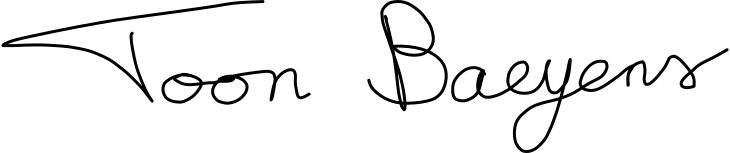
\includegraphics[width=4cm]{img/signature.pdf}\\
    June 2023
\end{flushright}

\stopchapter



% !TeX root = chapter_software.tex
% !TeX root = thesis.tex
\ifdefined\UtilIncluded
  \renewcommand{\startchapter}[1]{}
  \renewcommand{\stopchapter}{}
\else

\newcommand{\startchapter}[1]{\begin{document}\setcounter{chapter}{#1}\addtocounter{chapter}{-1}}
\newcommand{\stopchapter}{\end{document}}


\documentclass[a4paper]{book}
\usepackage[utf8]{inputenc}

\usepackage{amsfonts,amsmath, amsthm, amssymb}
\usepackage{xspace}
\usepackage[hidelinks,bookmarks,pdfusetitle]{hyperref}
\usepackage{listings}
\usepackage[pdftex]{graphicx}
\usepackage{bm}
\usepackage[english]{babel}
\usepackage{caption}
\usepackage{subcaption}
\usepackage[usenames,dvipsnames]{xcolor}
\usepackage{physics}
\usepackage{multicol}
\usepackage{xstring}
\usepackage{pythonhighlight}
\usepackage{parskip}
\usepackage{thmtools}
\usepackage{relsize}
\usepackage{bookmark}
\usepackage{lmodern}
\usepackage{ifthen}
\usepackage{biblatex}
\usepackage{csquotes}

\addbibresource{references.bib}

\newtheorem{theorem}{Theorem}
\newtheorem{lemma}[theorem]{Lemma}
\newtheorem{corollary}[theorem]{Corollary}

\DeclareRobustCommand{\oneD}{{1{\relsize{-1}D}}\xspace}
\DeclareRobustCommand{\twoD}{{2{\relsize{-1}D}}\xspace}
\DeclareRobustCommand{\threeD}{{3{\relsize{-1}D}}\xspace}
\DeclareRobustCommand{\cpp}{{{C\nolinebreak[4]\hspace{-.05em}\raisebox{.4ex}{\relsize{-3}\textbf{++}}}\xspace}}
\pdfstringdefDisableCommands{%
    \def\cpp{C++}%
    \def\oneD{1D}%
    \def\twoD{2D}%
    \def\threeD{3D}%
}

\newcommand{\longchapter}[2][]{%
    \chapter[#2]{#2}%
    \ifthenelse{\equal{#1}{}}{}{\chaptermark{#1}}}

\fi
\gdef\UtilIncluded{}


\startchapter{0}

\undefinedlabel{cha:c2}{2}
\undefinedlabel{cha:c3}{3}
\undefinedlabel{cha:c4}{4}

\chapter*{Summary}
\addcontentsline{toc}{chapter}{Summary}


\section*{English summary}
\addcontentsline{toc}{section}{English summary}

An $n$-dimensional time-independent Schrödinger equation is a linear second order partial differential equation given by
\begin{equation}\label{equ:sum_en_schrodinger}
-\nabla^2 \psi(\vb{x}) + V(\vb{x}) \psi(\vb{x}) = E\vb{x}\text{.}
\end{equation}
In this expression, $V$ is a provided potential functions defined on the domain $\Omega \subseteq \RR^n$. When solving this equation, the goal is to find all functions $\psi : \Omega \to \RR$ and values $E \in \RR$ that satisfy the Schrödinger equation~\eqref{equ:sum_en_schrodinger} in combination with provided boundary conditions. In such a solution $E$ is called the eigenvalue, with corresponding eigenfunction $\psi$.

For the one-dimensional case, Schrödinger equations are a special case of Sturm--Liouville equations:
\begin{equation}\label{equ:sum_en_sl}
    -(p(x), y'(x))' + q(x) y(x) = \lambda w(x) y(x) \text{.}
\end{equation}
In this equation $p(x)$, $q(x)$ and $w(x)$ are given functions on a connected domain $[a, b] \subseteq \RR$. Here, $\lambda$ is the unknown eigenvalue with corresponding eigenfunction $y$.

In chapter \ref{cha:c2}, an existing numerical method for approximating eigenvalues and eigenfunctions of \eqref{equ:sum_en_sl} is studied. Here regular Sturm--Liouville problems on $[a, b]$ are considered with homogeneous Robin boundary conditions:
$$
\alpha_a y(a) + \beta_a p(a) y'(a) = 0 \text{ and } \alpha_b y(b) + \beta_b p(b) y'(b) = 0\text{.}
$$
This constant-perturbation method is able to reach extremely accurate results, for small as well as high eigenvalues.

\todo{Why is ours better?}

\todo{Two-dimensional problems.}

% LTeX: language=nl-BE
\section*{Nederlandse samenvatting}
\addcontentsline{toc}{section}{Nederlandse samenvatting}


\stopchapter


% !TeX root = chapter_software.tex
% !TeX root = thesis.tex
\ifdefined\UtilIncluded
  \renewcommand{\startchapter}[1]{}
  \renewcommand{\stopchapter}{}
\else

\newcommand{\startchapter}[1]{\begin{document}\setcounter{chapter}{#1}\addtocounter{chapter}{-1}}
\newcommand{\stopchapter}{\end{document}}


\documentclass[a4paper]{book}
\usepackage[utf8]{inputenc}

\usepackage{amsfonts,amsmath, amsthm, amssymb}
\usepackage{xspace}
\usepackage[hidelinks,bookmarks,pdfusetitle]{hyperref}
\usepackage{listings}
\usepackage[pdftex]{graphicx}
\usepackage{bm}
\usepackage[english]{babel}
\usepackage{caption}
\usepackage{subcaption}
\usepackage[usenames,dvipsnames]{xcolor}
\usepackage{physics}
\usepackage{multicol}
\usepackage{xstring}
\usepackage{pythonhighlight}
\usepackage{parskip}
\usepackage{thmtools}
\usepackage{relsize}
\usepackage{bookmark}
\usepackage{lmodern}
\usepackage{ifthen}
\usepackage{biblatex}
\usepackage{csquotes}

\addbibresource{references.bib}

\newtheorem{theorem}{Theorem}
\newtheorem{lemma}[theorem]{Lemma}
\newtheorem{corollary}[theorem]{Corollary}

\DeclareRobustCommand{\oneD}{{1{\relsize{-1}D}}\xspace}
\DeclareRobustCommand{\twoD}{{2{\relsize{-1}D}}\xspace}
\DeclareRobustCommand{\threeD}{{3{\relsize{-1}D}}\xspace}
\DeclareRobustCommand{\cpp}{{{C\nolinebreak[4]\hspace{-.05em}\raisebox{.4ex}{\relsize{-3}\textbf{++}}}\xspace}}
\pdfstringdefDisableCommands{%
    \def\cpp{C++}%
    \def\oneD{1D}%
    \def\twoD{2D}%
    \def\threeD{3D}%
}

\newcommand{\longchapter}[2][]{%
    \chapter[#2]{#2}%
    \ifthenelse{\equal{#1}{}}{}{\chaptermark{#1}}}

\fi
\gdef\UtilIncluded{}


\startchapter{0}

\undefinedlabel{cha:c2}{2}
\undefinedlabel{cha:c3}{3}
\undefinedlabel{cha:c4}{4}

\chapter*{Developed software}
\addcontentsline{toc}{chapter}{Overview of developed software}
\markboth{Developed software}{Developed software}

All developed software consists of \cpp{}-source files together with a \lpython{}-package. This \lpython{}-package provides a user-friendly interface to the efficiently implemented \cpp{}-code. To build upon this code, \lpython{} is an optional dependency. All Schrödinger problems can also be expressed using only \cpp{}.

\subsection*{Matslise 3.0 --- pyslise}

Solving one-dimensional Sturm--Liouville and Schrödinger problems with homogenous Robin or periodic boundary conditions. See chapter~\ref{cha:c2}.

\url{https://github.com/twist-numerical/matslise} \\
\url{https://pypi.org/project/pyslise/}


\subsection*{Matslise 2D --- pyslise2d}

Approximating eigenvalues and eigenfunctions of two-dimensional Schrödinger problems on rectangular domains with homogenous Dirichlet boundary conditions, using the method from chapter~\ref{cha:c3}.

\url{https://github.com/twist-numerical/matslise2d} \\
\url{https://pypi.org/project/pyslise2d/}


\subsection*{Strands --- strands}

Approximating eigenvalues and eigenfunctions of two-dimensional Schrödinger problems on general bounded domains with homogenous Dirichlet boundary conditions, using the method from chapter~\ref{cha:c4}.

\url{https://github.com/twist-numerical/strands} \\
\url{https://pypi.org/project/Strands/}


\stopchapter


% !TeX root = chapter1_introduction.tex
% !TeX root = thesis.tex
\ifdefined\UtilIncluded
  \renewcommand{\startchapter}[1]{}
  \renewcommand{\stopchapter}{}
\else

\newcommand{\startchapter}[1]{\begin{document}\setcounter{chapter}{#1}\addtocounter{chapter}{-1}}
\newcommand{\stopchapter}{\end{document}}


\documentclass[a4paper]{book}
\usepackage[utf8]{inputenc}

\usepackage{amsfonts,amsmath, amsthm, amssymb}
\usepackage{xspace}
\usepackage[hidelinks,bookmarks,pdfusetitle]{hyperref}
\usepackage{listings}
\usepackage[pdftex]{graphicx}
\usepackage{bm}
\usepackage[english]{babel}
\usepackage{caption}
\usepackage{subcaption}
\usepackage[usenames,dvipsnames]{xcolor}
\usepackage{physics}
\usepackage{multicol}
\usepackage{xstring}
\usepackage{pythonhighlight}
\usepackage{parskip}
\usepackage{thmtools}
\usepackage{relsize}
\usepackage{bookmark}
\usepackage{lmodern}
\usepackage{ifthen}
\usepackage{biblatex}
\usepackage{csquotes}

\addbibresource{references.bib}

\newtheorem{theorem}{Theorem}
\newtheorem{lemma}[theorem]{Lemma}
\newtheorem{corollary}[theorem]{Corollary}

\DeclareRobustCommand{\oneD}{{1{\relsize{-1}D}}\xspace}
\DeclareRobustCommand{\twoD}{{2{\relsize{-1}D}}\xspace}
\DeclareRobustCommand{\threeD}{{3{\relsize{-1}D}}\xspace}
\DeclareRobustCommand{\cpp}{{{C\nolinebreak[4]\hspace{-.05em}\raisebox{.4ex}{\relsize{-3}\textbf{++}}}\xspace}}
\pdfstringdefDisableCommands{%
    \def\cpp{C++}%
    \def\oneD{1D}%
    \def\twoD{2D}%
    \def\threeD{3D}%
}

\newcommand{\longchapter}[2][]{%
    \chapter[#2]{#2}%
    \ifthenelse{\equal{#1}{}}{}{\chaptermark{#1}}}

\fi
\gdef\UtilIncluded{}


\startchapter{1}

\undefinedlabel{cha:c2}{2}
\undefinedlabel{cha:c3}{3}
\undefinedlabel{cha:c4}{4}

\chapter{Introduction to differential equations}

Differential equations recall in most mathematicians many feelings. Some only shiver by the mere idea of them, some of my colleagues in the more algebraic, (finite) geometric or discrete fields come to mind. Others, myself included, rejoice at the thought of studying them.

The knowledge about and experience with differential equations vary wildly among, even the best of, mathematicians. Some only had one, maybe two, introductory courses, others have studied them their whole careers. Important note: there are very few mathematicians that can say they have studied `differential equations'. Neither can I, I have studied \emph{a} differential equation. Maybe two, if you count generously.

Before diving into the required mathematical background, let us take a step back. Mathematics does not live in a vacuum. Modern ideas have grown out of a very rich history, with many influences from the scientific questions of the time. In this introduction we will take the time to appreciate this history, and discover how differential equations have been developed.

\section{History}

In this section, we will walk through an abridged version of the history of differential equations. Before talking about functions, it is important to talk about what makes up these functions.

A good starting point is to take a look at numbers. Counting things is universal and timeless, as such the natural numbers $\NN$ are a jumping point to all the other numbers. In modern mathematics, the next logical step is to introduce the integers $\ZZ$. But historically, negative numbers, and the concept of zero as a number, were only widely accepted throughout the Middle Ages, by Indian, Chinese and Arabic mathematicians.

In historic texts, we find already references to (positive) fractions, as early as Ancient Egypt, around 1000 BC. So after $\NN$ the next numbers that were `discovered', were the positive rational numbers $\QQ^+$. And soon thereafter some irrational numbers were found. The most prominent example is probably $\sqrt{2}$, the length of the diagonal of the unit square. But it is a bit too generous to say that this was the discovery of the real numbers. It is more accurate to say that there was a notion of algebraic numbers $\QQbar$. These are the numbers that are solutions of polynomial equations, like $x^2 = 2$. But only around the year 900, the Egyptian mathematician Abū Kāmil Shujā ibn Aslam started to accept these solutions as numbers in and of itself.

The mathematical invention that may have had the most impact in our daily lives, may also be unnoticed by many: the Hindu--Arabic numeral system. This is a way of writing down numbers, invented between the first and fourth century. Most numeral systems were not made for large numbers or were cumbersome to work with. Only the best of mathematicians could do computation in those systems, especially multiplication was difficult. The Hindu--Arabic numeral system solved this by being positional based. This means that the last digits is the one's place, the digit before that ten's, then hundred's, and so on. This allows for a compact way to write down large numbers, that still allows easy computation through arithmetic manipulations. Our modern numeral system is a direct descendant of the Hindu--Arabic numeral system. Compare for example the Roman numeral \uppercase\expandafter{\romannumeral 3846\relax} to our modern equivalent $3846$. And to help illustrate this point, try squaring both numbers.

From the sixteenth century onwards mathematics in Europe started to flourish. For our purposes, the next stride towards the real numbers was made by Simon Stevin from Bruges. He created a way to write real numbers as a decimal expansion. It was Stevin who introduced the concept of `digits behind the decimal point'. In this same century the complex numbers were discovered. And later in 1637, it was René Descartes who coined the terms `real' and `imaginary' numbers.

But it still took more than 200 years more before we would get a first formal mathematical definition of the real numbers $\RR$. It was the work of the great logicians of the late 19th century, spearheaded by Georg Cantor. He provided in 1874 a formal logical construction of the real numbers. It may seem surprising that a rigorous definition of the real numbers came so late in the rich history of mathematics. But, in practice, the development of calculus, and the theory of functions, did not really require strict formal definitions to advance.

\subsection{Calculus}

From a natural sciences view, it is natural to study relations between quantities. For example position in function of time, or air resistance in function of velocity. Yet, the earliest examples of the use of calculus seem to have their origins in geometry: finding the area under a parabola, or the volume of a cone\dots

Throughout Ancient times and the Middle Ages across mathematical texts of many cultures, diverse examples of what we now call derivatives and integrals can be found. But all these examples were concrete applications to problems. Only in the seventeenth century were the first unifying theories of derivatives and integrals of functions developed. It was by non-other than Newton and Leibniz. The history between these two fathers of calculus is much richer than one would expect, it reads almost as a screenplay. In short, it is now accepted that both mathematicians independently developed the theory of calculus, at the time it was not.

The notations
$$
    \int f(x) \, \dd x \quad \text{ and } \dv[]{f(x)}{x}
$$
for the integral and the derivative of a function $f$ were introduced by Liebniz. Newton introduced the notation
$$
    \dot{f}
$$
for the derivative of $f$. In mathematical texts this notation is less common, but it can be abundantly found in physics. In this work we will mostly use $\dv[]{f}{x}$ for the derivative of $f$. If from context the variable to which the derivative is considered is clear, then we will abbreviate $\dv[]{f}{x}$ to $f'(x)$.

For many examples of how the theory of calculus and especially differential equations have developed throughout the last 400 years, we refer the interested reader to \cite{archibald_history_2005}. One of these examples explains what Newton probably understood by integrals and quadratures, and how these were computed. Another example is concerned with how the works of d'Alembert evolved.

The first differential equations, as we know them now, were studied shortly after the work by Newton. Leibniz himself, and the Bernoulli brothers came across differential equations in the context of geometry and mechanics. In the eighteenth century the multivariate theory of Leibniz was extended and the first partial differential equations were written down. In the nineteenth century from the theoretical side, more results about the existence of solutions to differential equation were found. From the practical side, many more applications were found. Not only in mechanics, but also in heat transfer, optics, fluid flow and electricity and magnetism were differential equations instrumental. The equations of Navier and Stokes or the laws of Maxwell, to name a few, were developed.

And the developments from the nineteenth century continued into the twentieth. Great new theoretical stride were made, and many new applications were found. Most notably, for this thesis at least, in quantum mechanics with Schrödinger's equation.

\subsection{Advent of computing}

Most\footnote{Mathematically, we can even say `almost all'.} differential equation can not be explicitly solved. For ordinary linear differential equations with constant coefficients, for example, symbolic results are available. But if one of the coefficients is not a constant, these formulae fail. For this reason, numerical methods for differential equations were developed. These methods do not solve the equation in the strictest sense, but they are able to approximate solutions arbitrarily accurate. The first numerical method is Euler's\footnote{Both forward and backward.} method from 1768. This is a simple method, yet Cauchy proved convergence. This convergence assures, that if sufficiently small steps are taken, any accuracy for the approximated solution can be obtained.

Later, in the middle of the nineteenth century multistep methods were developed. And at the end of that century, Runge published the first Runge--Kutta method. These `new' methods were of higher order than the simpler methods and therefore could take larger steps to reach sufficiently accurate results.

What strikes me the most is that all these methods were developed long before computers were invented. This implies that the first applications of these methods required an unfathomable amount of manual computation. Now, we are spoiled, and computers do all the numerical heavy lifting for us\footnote{Regularly I feel very fortunate to be a PhD-student now, and not then. I assume that, before computers, many tedious computations must have been assigned to students.}. Back then, the term `computer' did exist, but it was a profession, not a device.

Throughout the twentieth century, with the rise of computing devices, the use and applicability of these numerical methods for ordinary differential equations exploded. We were able to reach never before-seen accuracies in fractions of the time it would have costed only a few decades earlier. This explosion in computational power has continued. Now, the speed of affordable consumer desktop computers can be measured in teraFLOPS\footnote{`FLOPS' is a measure of how many \emph{fl}oating point \emph{o}perations \emph{p}er \emph{s}econd a computer can execute. A computer with a speed of $1$ teraFLOPS can execute  one billion floating point operations each second.}. For example, my university computer (Intel i7-8700K and an NVIDIA Quadro P2000) has a combined rated speed of a little over 3 teraFLOPS. Almost all of this speed comes from its graphics processing unit, with the CPU only contributing $0.06$ teraFLOPS. This already indicates that FLOPS is an imperfect unit. Writing a program that is able to use \emph{all} these FLOPS is prohibitively difficult.

\section{Ordinary differential equations}

In the most general formulation, an $n$-dimensional $k^\text{th}$ order ordinary differential equation 
$$
f\left(x, y, {\pdv[]{y}{x}}, {\pdv[2]{y}{x}}, \dots, {\pdv[k]{y}{x}}\right) = 0
$$
expresses a constraint on an unknown sufficiently differentiable function $y : \Omega \to \RR$ with $\Omega \subseteq \RR$ and $f: \RR^{k+1} \to \RR$. In most cases, this equation alone is unsufficient to determine a unique solutions $y(x)$. For this, some initial or boundary conditions can be imposed on $y$ (or any of the derivatives). As this abstract description is not intuitive, we provide some examples.

\paragraph{Integrals} The problem of determining primitive functions $F(x)$ can be rewritten as an ordinary differential equation:
$$
F(x) = \int f(x) \,\dd x \quad \iff \quad \dv[]{F}{x} = f(x)\text{.}
$$
Definite integrals can similarly be formulated as an ordinary differential, however a boundary condition has to be imposed:
$$
\int_a^b f(x) \dd x = F(b) \quad \text{ with } \dv[]{F}{x} = f(x) \text{ and } F(a) = 0\text{.}
$$

Mathematically, this is a valid example. Intuitively however, this seems rather trivial.

\paragraph{Swinging pendulum} Due to Newton's laws of motion, physical system often give rise to second order ordinary differential equations. One such example is a pendulum. Here, a mass is suspended such that it can swing freely back and forth. Let $\theta(t)$ be the angle by which the mass is displaced from its hanging resting position at time $t$. The movement of the pendulum is described by
$$
\dv[2]{\theta}{t} + \frac{g}{l} \sin(\theta) = 0\text{,}
$$
with $g$ the gravitational constant, and $l$ the distance between the fixed point and the mass. As initial conditions at time $t_0$, $\theta(t_0)$ represents the displacement angle at $t_0$ and $\theta'(t_0)$ represents some initial angular velocity with which the mass is released.

\paragraph{Brachistochrone curve} Mathematicians love challenging each other. This is true today, as much as it was 300 years ago. In 1696 posed Johann Bernoulli the Brachistochrone problem: on which curve slides a frictionless bead the fastest from point $A$ to $B$? There are many strategies for solving this problem. In one such solutions, the following differential equation arises:
$$
{\dv[]{y}{x}} = \sqrt{\frac{D - y}{x}} \text{ with $y(0) = 0$,}
$$
with $D$ a parameter.

\paragraph{Lotka--Volterra equations} In biological modelling, dynamical systems can describe many real-world situations. One such a system are the Lotka-Volterra equations. This set of equations models the population size of two species. One function $r(t)$ expresses the population size of prey (for example rabbits), the other function $f(t)$ tracks the population size of de predatory species (for example foxes). The Lotka--Volterra equations are
$$
\begin{cases}
    \dv[]{x}{t} = \alpha x - \beta x y \\
    \dv[]{y}{t} = \delta x y - \gamma y \\
\end{cases}\text{.}
$$
The constants $\alpha$, $\beta$, $\gamma$ and $\delta$ are parameters which describe the particular siituation under study. Typically, as initial conditions a researchers suplies the population sizes of both species at the start of the simulation.

\subsection{Sturm--Liouville problems}

These were only a few short examples from a myriad of real-world applications. In chapter \ref{cha:c2} we will focus upon the numerical solution of a particular class of second-order linear ordinary differential equation: Sturm--Liouville equations.

A Sturm--Liouville problem is defined by three functions $p(x)$, $q(x)$ and $w(x)$ on a domain $\Omega \subseteq \RR$.
$$
-{\dv[]{}{x}}\left(p(x) \dv[]{y}{x}\right) + q(x) y = \lambda w(x) y
$$
This problem is only well-defined if appropriate boundary condtions are provided as well. For more details about differnent types of boundary conditions we refer the reader to the introduction in chapter \ref{cha:c2}.

One striking particularity of these problems is that, besides $y(x)$, $\lambda$ is an unknown as well. Solutions for $\lambda$ are called eigenvalues and the corresponding solution for $y(x)$ is what is called an eigenfunction. 

Differential equations can be approached from many different angles. Some researchers take a pure theoretical approach, where many powerful results are proven. Other researchers start with real-world applications and consider differential equations as simply a tool in there toolbox to tackle their problems. The approach we have chosen falls somewhere in between. From the beginning we set out to develop and implement numerical methods for particaular differential equations. To build a useful and accuracte method, many theoretical results are needed. However, also practical feasibility and computational efficiency are essential\footnote{Personally, I feel this is the true strength of this thesis. Neither the theoretical advancements we made, nor the efficiency of our implementation are perfect. However, I believe the powerfull combination of the two to be the real innovation.}.


\section{Partial differential equations}



\subsection{Time-dependent problems}

\subsection{Eigenvalue-eigenfunction problems}

\stopchapter


% !TeX root = chapter2_1d.tex
% !TeX root = thesis.tex
\ifdefined\UtilIncluded
  \renewcommand{\startchapter}[1]{}
  \renewcommand{\stopchapter}{}
\else

\newcommand{\startchapter}[1]{\begin{document}\setcounter{chapter}{#1}\addtocounter{chapter}{-1}}
\newcommand{\stopchapter}{\end{document}}


\documentclass[a4paper]{book}
\usepackage[utf8]{inputenc}

\usepackage{amsfonts,amsmath, amsthm, amssymb}
\usepackage{xspace}
\usepackage[hidelinks,bookmarks,pdfusetitle]{hyperref}
\usepackage{listings}
\usepackage[pdftex]{graphicx}
\usepackage{bm}
\usepackage[english]{babel}
\usepackage{caption}
\usepackage{subcaption}
\usepackage[usenames,dvipsnames]{xcolor}
\usepackage{physics}
\usepackage{multicol}
\usepackage{xstring}
\usepackage{pythonhighlight}
\usepackage{parskip}
\usepackage{thmtools}
\usepackage{relsize}
\usepackage{bookmark}
\usepackage{lmodern}
\usepackage{ifthen}
\usepackage{biblatex}
\usepackage{csquotes}

\addbibresource{references.bib}

\newtheorem{theorem}{Theorem}
\newtheorem{lemma}[theorem]{Lemma}
\newtheorem{corollary}[theorem]{Corollary}

\DeclareRobustCommand{\oneD}{{1{\relsize{-1}D}}\xspace}
\DeclareRobustCommand{\twoD}{{2{\relsize{-1}D}}\xspace}
\DeclareRobustCommand{\threeD}{{3{\relsize{-1}D}}\xspace}
\DeclareRobustCommand{\cpp}{{{C\nolinebreak[4]\hspace{-.05em}\raisebox{.4ex}{\relsize{-3}\textbf{++}}}\xspace}}
\pdfstringdefDisableCommands{%
    \def\cpp{C++}%
    \def\oneD{1D}%
    \def\twoD{2D}%
    \def\threeD{3D}%
}

\newcommand{\longchapter}[2][]{%
    \chapter[#2]{#2}%
    \ifthenelse{\equal{#1}{}}{}{\chaptermark{#1}}}

\fi
\gdef\UtilIncluded{}


\startchapter{2}

\longchapter[The \oneD Schrödinger equation]{The one-dimensional time-independent Schrödinger equation}\label{cha:c2}

\section{Introduction}

The one-dimensional time-independent Schrödinger equation is an eigenvalue problem with boundary conditions. Solutions are given as an eigenvalue $\lambda \in \RR$ with corresponding eigenfunction $y: \RR \to \RR$. These eigenfunctions are defined over the bounded domain $[a, b] \subseteq \RR$ of the problem. Each solution has to satisfy the following equation
$$
    -y''(x) + V(x)y(x) = \lambda y(x)
$$
for each of the values $x\in [a, b]$. In this equation the given function $V: \RR \to \RR$ is the potential of the problem at hand. Note that in general if $y(x)$ is an eigenfunction, $c\,y(x)$ will also be an eigenfunction with the same eigenvalue, for each value of $c \in \RR$. As such, it is not really possible to say ``\emph{the} eigenfunction of corresponding to a certain eigenvalue". Later on we will prove that in many cases the eigenfunction is, up to a constant factor, uniquely defined.

Boundary conditions have to be specified before solutions can be found. These conditions pose restrictions on $y(a)$, $y'(a)$, $y(b)$ and $y'(b)$. Boundary conditions come in many flavors. We provide an overview of the most common ones:
\begin{itemize}
    \item \emph{Dirichlet boundary conditions} specify which value the solution takes on the boundary of the domain. In our case, eigenfunctions can always be scaled, as such, it is not useful to specify the value of the solution different from zero on the boundary. This type of boundary condition thus simplifies to $y(a) = 0$ and $y(b) = 0$.
    \item \emph{Neumann boundary conditions} specify which value the derivative of a solution takes on the boundary of the domain. In our case, the same remark as given for the Dirichlet boundary conditions applies. This means that Neumann boundary conditions imply that $y'(a) = 0$ and $y'(b) = 0$.
    \item \emph{Robin boundary conditions} are a generalization of both previous boundary conditions. When these conditions are imposed on a solution $y(x)$ we imply that a certain weighted average of the function and its derivative are a fixed value. As solutions can always be scaled, Robin boundary conditions can be, in our case, rewritten to
          $$
              \alpha_a y(a) + \beta_a y(a) = 0 \text{ and } \alpha_b y(b) + \beta_b y(b) = 0  \text{.}
          $$
    \item \emph{Periodic boundary conditions} are used to specify that a solution should be periodic. In other words, the solutions has to end in the same value as it started, and so should the derivative. Mathematically this can be written as: $y(a) = y(b)$ and $y'(a) = y'(b)$. These condition can be extended to \emph{anti-periodic boundary conditions}: $y(a) = -y(b)$ and $y'(a) = -y'(b)$. Or even generalized to
          $$
              \begin{pmatrix} y(a) \\ y'(a) \end{pmatrix} = \vb{K} \begin{pmatrix} y(b) \\ y'(b) \end{pmatrix}\text{.}
          $$
\end{itemize}

Note that Dirichlet or Neumann boundary conditions can always be written as Robin boundary conditions. So when studying the one-dimensional time-independent Schrödinger equation it is most general to always consider Robin boundary conditions. Periodic (or generalized periodic) boundary conditions are less common and give rise to more edge cases and subtleties. This case will be later studied in section \ref{sec:1d_periodic}.

\subsection{Properties of the Sturm-Liouville equation}

Before developing numerical methods for solving these equations it is important to build a strong theoretical foundation. The goal is to build a thorough understanding of the Schrödinger equation and use this intuition to develop efficient and accurate numerical algorithms to solve this equation.

In the scientific literature it is quite rare to find studies about the one-dimensional Schrödinger equation itself. Most, if not all, articles and books cover the more general Sturm-Liouville theory. As Sturm-Liouville equations are a generalization of Schrödinger equations they are more wildly applicable, and so more useful to study. In this section, we will follow the tradition from the literature and study the Sturm-Liouville equation. Many more details and examples of the Sturm-Liouville theory can be found in relevant textbooks, for example \cite[Chapter~5]{sagan_boundary_1961}.

The Sturm-Liouville equation is a boundary value eigenproblem, given by the following equation on the bounded domain $[a, b]$
$$
    -(p(x) y'(x))' + q(x) y(x) = E w(x) y(x)\text{.}
$$
The continuous and finite functions $p(x)$, $q(x)$ and $w(x)$ are given on the domain. These functions define the problem. A solution consists of an eigenvalue $E$ with corresponding eigenfunction $y(x)$. For now, we will study the Sturm-Liouville equation with Robin boundary conditions:
$$
    \alpha_a y(a) + \beta_a p(a) y'(a) = 0 \text{ and } \alpha_b y(b) + \beta_b p(b) y'(b) = 0\text{.}
$$

Note that the Schrödinger equation with Robin boundary conditions is a special case of the Sturm-Liouville equation. Namely, when $p(x) = 1$, $q(x) = V(x)$ and $w(x) = 1$.

    {\color{red}

        Following from the mathematical background chapter:
        \begin{itemize}
            \item Eigenvalues are real and ordered.
            \item Eigenfunctions can be orthonormal
        \end{itemize}

        In finite and non-periodic cases: eigenvalues are unique.

        \subsection{Liouville's transformation}
        Liouville provided, under certain conditions, a transformation to reduce the Sturm-Liouville equation back to the Schrödinger equation. This transformation can be used to employ the easier numerical algorithms for Schrödinger equations, to solve more general Sturm-Liouville equations.

    }



\section{Background about Matslise}

Numerical methods for ordinary differential equations as \emph{initial value} problems are already more than a century old. In particular, linear multistep methods and Runge-Kutta methods were described around 1900. First they were applied and calculated by hand, later on ``calculating machines'' \cite{milne_numerical_1926} were used. Nowadays, modern computers do all the tedious computations.

For ordinary differential equations as \emph{boundary value} problems, such as the Sturm-Liouville equations, the story is different. There still are very few general methods for such problems. For linear ordinary differential equations, one of the more popular choices is a method based upon finite differences.

\begin{figure}
    \begin{center}
        \includegraphics[width=\textwidth]{img/chapter2/finite_difference_grid.pdf}
    \end{center}
    \caption{An equidistant division of the domain $[a, b]$ in $n$ intervals.}
    \label{fig:c2_finite_difference_grid}
\end{figure}

The idea for these kinds of methods, is to discretize the integration domain $[a, b]$ into an equally spaced grid of points $a = x_0$, $x_1$, $\dots$, $x_i$, $\dots$, $x_{n-1}$, $x_{n} = b$, with $\Delta x$ the distance between two consecutive points. This discretization can be seen in figure \ref{fig:c2_finite_difference_grid}. The differential equation is now approximated by using finite difference expressions of the involved derivatives. This leads to a linear matrix-vector reformulation of the differential equation, which can be solved with classical linear algebra tools.

\subsubsection{Finite difference approximation of the Sturm-Liouville equation}

Around 1990 the best methods \cite{andrew_correction_1985,vandenberghe_accurate_1991} for approximating solutions to the Sturm-Liouville equation looked at the simpler form of the Schrödinger equation and apply. After the fact, they applied some corrections to improve the accuracy of higher eigenvalues. They experimented with which finite difference approximations to use. First they tried classical formulae,  later they developed highly tuned exponential fitted formulae to better handle the oscillatory nature of the eigenfunctions.

To illustrate this class of finite difference methods for Sturm-Liouville equations we will develop a simpler version ourselves. This will allow us to appreciate the nuances of these methods more, and it will give us some ideas about the general disadvantages of this technique. The Sturm-Liouville equations we will consider are given by
\begin{equation}\label{equ:c2_finite_difference_slp}
    -(p(x)y')' + q(x) y = \lambda w(w) y\text{.}
\end{equation}
Solutions consist of eigenvalues $\lambda$ and corresponding eigenfunctions $y(x)$ such that \eqref{equ:c2_finite_difference_slp} is satisfied on the domain $[a, b]$ with homogeneous Dirichlet boundary conditions $y(a) = y(b) = 0$.

As a first step we discretize the domain $[a, b]$ with $n+1$ equidistant points, as in figure \ref{fig:c2_finite_difference_grid}. The eigenfunctions $y(x)$ we are looking for, can now be approximated by values in each of the grid points $y(x_i) \approx y_i$. For translating this problem into a linear matrix-vector equation, we are missing one key component. We still need a way to discretize the expression $(p(x) y')'$. For this, we apply the central second order finite difference formula for the first derivative twice, with half the step size. In more detail, the first derivative of a scalar function $f(x)$ can be approximated as:
$$
    f'(x) \approx \frac{f(x + h) - f(x - h)}{2h}\text{.}
$$

Applying this expression once to $(p(x) y')'$ in the point $x_i$, with step size $h = \frac{\Delta x}{2}$ gives:
$$
    (p(x) y')'(x_i) \approx \frac{1}{\Delta x}\left((p y')\left(x_{i+\frac{1}{2}}\right) - (p y')\left(x_{i-\frac{1}{2}}\right))\right)\text{.}
$$
Applying the finite difference formula a second time, with step size $\frac{\Delta x}{2}$ to approximate $y'(x)$ yields:
$$
    (p(x) y')'(x_i) \approx \frac{1}{\Delta x^2}\left(p_{i+\frac{1}{2}} y_{i+1} - \left(p_{i-\frac{1}{2}} + p_{i+\frac{1}{2}}\right) y_i + p_{i-\frac{1}{2}} y_{i-1}\right)
$$
To ease notation we have substituted $y(x_i)$ with its approximation $y_i$, and have denoted $\frac{x_i + x_{i+1}}{2}$ as $x_{i+\frac{1}{2}}$, and $p(x_i)$ as $p_i$. Also, note that if $p(x) = 1$ this formula simplifies to the classical, well-known, central second order approximation of the second derivative.

If we apply this finite difference approximation to \eqref{equ:c2_finite_difference_slp} in each point $x_i$. We get the linear generalized eigenvalue problem:
$$
    -\frac{1}{\Delta x^2}\left(p_{i+\frac{1}{2}} y_{i+1} - \left(p_{i-\frac{1}{2}} + p_{i+\frac{1}{2}}\right) y_i + p_{i-\frac{1}{2}} y_{i-1}\right) + q(x_i) y_i = \lambda w(x_i) y_i \text{.}
$$

To emphasize that this is a linear algebra problem we can rewrite this in matrix notation:
\begin{equation}\label{equ:c2_finite_difference_matrix_problem}
    \left(-\vb{D} + \diag(\vb{q})\right)\vb{y} = \lambda \diag(\vb{w}) \vb{y}\text{.}
\end{equation}

The $(n-1)$-dimensional vector $\vb{y} = \transpose{\begin{pmatrix}y_1 & y_2 & \dots & y_{n-1}\end{pmatrix}}$ is the unknown approximation of the eigenfunction. The $(n-1)$-dimensional vectors $\vb{q} = \transpose{\begin{pmatrix}q(x_1) & q(x_2) & \dots & q(x_{n-1})\end{pmatrix}}$  and $\vb{w} = \transpose{\begin{pmatrix}w(x_1) & w(x_2) & \dots & w(x_{n-1})\end{pmatrix}}$ are the values of the coefficient functions $q$ and $p$. And lastly, the matrix $\vb{D}$ is the tridiagonal matrix given by:
$$
    \vb{D} = \frac{1}{\Delta x^2}\begin{pmatrix}
        -p_{\frac{1}{2}} -p_{\frac{3}{2}} & p_{\frac{3}{2}}                   &                                   &                     &                                            \\
        p_{\frac{3}{2}}                   & -p_{\frac{3}{2}} -p_{\frac{5}{2}} & p_{\frac{5}{2}}                   &                     &                                            \\
                                          & p_{\frac{5}{2}}                   & -p_{\frac{5}{2}} -p_{\frac{7}{2}} & p_{\frac{7}{2}}     &                                            \\
                                          &                                   &                                   & \ddots              &                                            \\
                                          &                                   &                                   & p_{n - \frac{3}{2}} & -p_{n - \frac{3}{2}} - p_{n - \frac{1}{2}} \\
    \end{pmatrix}{}\text{.}
$$

To find the eigenvalues of \eqref{equ:c2_finite_difference_matrix_problem} one can notice that if $w(x_i)$ is never $0$ for $0 < i < n$ then $\diag(\vb{w})$ is invertible and the problem becomes a simple tridiagonal eigenvalue problem. This can then be solved with our favorite tridiagonal eigenvalue solver. If $w$ happens to be constant, this becomes a symmetric tridiagonal matrix, for which LAPACK \cite{lapack}, for example, contains the specialized routines: \texttt{?stev} and relatives.

\begin{figure}
    \begin{center}
        \includegraphics[width=\textwidth]{img/chapter2/finite_difference_h_error.pdf}
    \end{center}
    \caption{Relative error of approximated eigenvalues of problem \eqref{equ:c2_fd_test_problem} in function of the grid size $n$ on the domain.}
    \label{fig:c2_fd_h_error}
\end{figure}

\begin{figure}
    \begin{center}
        \includegraphics[width=\textwidth]{img/chapter2/finite_difference_k_error.pdf}
    \end{center}
    \caption{Relative error of approximated eigenvalues of problem \eqref{equ:c2_fd_test_problem} in function of the eigenvalue index $k$.}
    \label{fig:c2_fd_k_error}
\end{figure}

As a numerical experiment of this method we will take a look at the following Sturm-Liouville equation:
\begin{equation}\label{equ:c2_fd_test_problem}
    -\left((1+x)^2 y \right)' + (x^2 - 2) y = \lambda e^x y
\end{equation}
on the domain $[0, 1]$ with homogeneous Dirichlet boundary conditions. Figure \ref{fig:c2_fd_h_error} shows the relative errors of the 4 lowest eigenvalues in function of the chosen grid size $n$. As $n$ increases, the error decreases, as desired. Notice that as the constructed method is based upon second order finite difference formulae, we expect to see the decrease of error be of second order too, as indicated in the figure with the dotted line. This constructed method is of relatively low order, so to compute very accurate estimations, a large grid size is needed. In the literature one can find many such methods, even with much higher orders. These better methods can reach high accuracy with relatively little computational work, for the first few eigenvalues.

As earlier hinted, this type of method struggles with the computation of higher eigenvalues. Figure \ref{fig:c2_fd_k_error} illustrates this. Here, the relative error of the first 50 eigenvalues is plotted, for different values of $n$. Note that in the case of $n = 32$, only $32$ eigenvalues can be computed. On this figure, the line corresponding to $\mathcal{O}(k^2)$ is drawn. Together with the $\mathcal{O}(\Delta x^2)$ from earlier, this indicates that the relative error of the $k^\text{th}$ eigenvalue is expected to be
$$
    \mathcal{O}(\Delta x^2 k^2)
$$
for this method applied to problem \eqref{equ:c2_fd_test_problem}. This teaches us, for this method in particular, but also applies to all methods of this type, that the larger the eigenvalue, the more difficult it is to compute accurately. In the literature one can find some techniques to mitigate this effect by applying some corrections after the fact. In \cite{andrew_correction_1985} such a correction is analyzed when applied to Numerov's method. Here, the authors are able to bring the error down from $\mathcal{O}(k^6 h^4)$ to $\mathcal{O}(k^3 h^4)$. This is remarkably better. But even with this correction technique, computing large eigenvalues is still computationally difficult.

\subsection{CP-methods}

The drawbacks of the methods based upon finite differences are already known for a long time. One of the first\footnote{In \cite{ledoux_solving_2010} a brief historical overview is given of the application of CP-methods to Sturm-Liouville problems. In this thesis we will take the time to take a closer look at the earlier methods. They will provide us a more intuitive understanding of the algorithms, in preparation of our own advancements within employing these ideas.} works that tries to not only mitigate these troubles but rather fully fix them, was \cite{canosa_new_1970} in 1970. There, Canosa and De Oliveira present a new method to approximate solutions to the one dimensional time-independent Schrödinger equation. This lays the foundation to what would later be called constant perturbation methods (CPM or CP-methods). To intuitively appreciate these CP-methods it is valuable to study the method from \cite{canosa_new_1970}.

For this, we will only consider the Schrödinger equation
\begin{equation}\label{equ:c2_cpm_schrodinger}
    - y'' + V(x) y = \lambda y
\end{equation}
on the domain $[a, b]$ with homogeneous Robin boundary conditions $\alpha_a y(a) + \beta_a y(a) = 0$ and $\alpha_b y(b) + \beta_b y(b) = 0$. But do note, that using Liouville's transformation all Sturm-Liouville problems can be transformed into Schrödinger problems.

\subsubsection{Piecewise constant approximation of the potential}

\begin{figure}
    \begin{center}
        \includegraphics[width=\textwidth]{img/chapter2/cpm_constant_approx.pdf}
        \caption{A potential function $V(x)$ is approximated as the piecewise constant function $\bar{V}(x)$ along the domain $[a, b]$.}
        \label{fig:c2_cpm_constant_approx}
    \end{center}
\end{figure}

As a very first step, \cite{canosa_new_1970} simplifies the potential $V(x)$ as a piecewise constant approximation $\bar{V}(x)$. This approximation is visualized in figure \ref{fig:c2_cpm_constant_approx}. Notice that no restrictions are placed upon the size of the pieces. Upon choosing $\bar{V}(x)$, one should keep in mind that the better the piecewise approximation is, the better the resulting eigenvalues will be. And, The computational runtime depends linearly on the number of pieces.

The next step is to fixate the value for $\lambda$. Now, for each of the pieces of $\bar{V}$ the analytical solutions is computed of the problem
$$
    y'' = (V_i - \lambda) y\text{.}
$$
Here, $V_i$ is the value of $\bar{V}$ on the $i^\text{th}$ piece $[x_i, x_{i+1}]$. These analytical solutions $\psi_i(x)$ have the following structure.
$$
    \psi_i(x) = \begin{cases}
        A_i + B_i x                                                         & \text{ if $V_i = \lambda$} \\
        A_i \cos(x\sqrt{\lambda - V_i}) + B_i \sin(x\sqrt{\lambda - V_i})   & \text{ if $V_i < \lambda$} \\
        A_i \cosh(x\sqrt{V_i - \lambda}) + B_i \sinh(x\sqrt{V_i - \lambda}) & \text{ if $V_i > \lambda$}
    \end{cases}
$$

To determine the appropriate values for $A_i$ and $B_i$ continuity conditions between pieces are applied:
$$
    \psi_{i-1}(x_i) = \psi_{i}(x_i) \text{ and } \psi_{i-1}'(x_i) = \psi_{i}'(x_i) \text{.}
$$
If $n$ pieces are used, this system of equations has $2n$ variables and $2(n-1)$ equations. Together with the two equations from the boundary conditions, this yields a fully determined linear system. To find eigenvalues $\lambda$ for which an eigenfunction exists such \eqref{equ:c2_cpm_schrodinger} is satisfied, the question now becomes: for which values of $\lambda$ does the previously described system of equations has non-zero solutions? Because only these solutions correspond to a non-zero eigenfunction.

Finding values for $\lambda$ for which the constructed system becomes singular is not as trivial as one may assume. In \cite{canosa_new_1970}, the authors have provided their own root finding algorithm based upon finding changes in the sign of the determinant. But this algorithm is not without issue. Eigenvalues may be arbitrarily close together, which makes it hard to ensure you have found all requested values. Choosing the appropriate step sizes when eigenvalues become increasingly sparse is a balance between efficiency and not missing any. Later on we will describe a way to reliably and efficiently determine all required eigenvalues.

One of the main benefits of this ``new method for the solution of the Schrödinger equation'' is that its accuracy does not depend on the size of the requested eigenvalue. Because only analytical solutions of the piecewise approximated problem are considered, oscillations can be represented exactly. Even the most extreme oscillations are cleanly captured inside the $\sin$ en $\cos$ of $\psi_i$. The idea of using analytical solutions allowed the development of the CP-methods.

When building upon this method one can make an observation when looking at figure \ref{fig:c2_cpm_constant_approx}. $\bar{V}(x)$ is a crude approximation of the function $V(x)$. This remark becomes even more important when one realizes that the accuracy of the method solely depends upon the accuracy of this approximation.

The idea of Canosa and De Oliveira gained traction. In 1971 Ixaru \cite{ixaru_error_1972} has written a note about the error analysis of this new method. And in the same year Pruess \cite{pruess_estimating_1973} has studied this method thoroughly and provided numerical examples of linear piecewise approximations and quadratic piecewise approximations of the potential function. Here we will state the most important theorems, without proof. All details can be found in \cite{pruess_estimating_1973}.

\begin{theorem}[Pruess 1973]\label{the:c2_pruess_1973_1}
    Let $\lambda_k$ be the $k^\text{th}$ eigenvalue of the Schrödinger equation
    $$
        -y'' + V(x) y = \lambda y
    $$
    on the domain $[a, b]$ with homogeneous Robin boundary conditions. And let $\tilde{\lambda}_k$ be the $k^\text{th}$ eigenvalue of the approximate Schrödinger equation with potential $\bar{V}(x)$ on the same domain, with identical boundary conditions. Here $\bar{V}(x)$ is a piecewise $m^\text{th}$ degree polynomial approximation, let $h$ be the width of the largest piece in this approximation. For $h$ sufficiently small, we have as $h \to 0$,
    $$
        |\lambda_k - \tilde{\lambda}_k| = \mathcal{O}(h^{2m + 2}) \text{ for each $k$.}
    $$
\end{theorem}

This theorem provides justification for the idea of Canosa and De Oliveira. Even though a constant approximation ($m = 0$) may be crude, it still is a second order method. Furthermore, the theorem suggest that expanding this method up to higher degree piecewise polynomial approximations may be worthwhile.

In \cite{pruess_estimating_1973}, the author also studies what happens to the error on the eigenvalues if $k$ is increased. In \cite{canosa_new_1970} it was assumed that this error does not get worse as $k$ increases.

\begin{theorem}[Pruess 1973]\label{the:c2_pruess_1973_2}
    Following the notation from theorem \ref{the:c2_pruess_1973_1}, assume $\bar{V}(x)$ to be a least squares $m^\text{th}$ degree piecewise polynomial approximation of $V(x)$. This means, on each piece $[x_i, x_{i+1}]$, that $\bar{V}$ is the $m^\text{th}$ degree polynomial such the following is minimal
    $$
        \int_{x_i}^{x_{i+1}} \left(V(x) - \bar{V}(x)\right)^2 \dd x \text{.}
    $$

    Under this assumption, if $k \to \infty$, it holds for the relative error that
    $$
        \frac{\lambda_k - \tilde{\lambda}_k}{\lambda_k} = \mathcal{O}(k^{-4})\text{.}
    $$
\end{theorem}

This last theorem does not only say that the error does not become larger if $k$ increases, but the relative error even decreases rapidly when $k \to \infty$. Theorem \ref{the:c2_pruess_1973_2} highlights the main advantage this technique has in comparison to other state-of-the-art methods. Where all other methods become less and less accurate for large eigenvalues, this method becomes even more accurate.

\begin{figure}
    \begin{center}
        \includegraphics[width=\textwidth]{img/chapter2/pruess_h_error.pdf}
    \end{center}
    \caption{Relative error of the found eigenvalues of problem \eqref{equ:c2_pruess_test_problem} by using the method of constant piecewise approximation of the potential, with equal pieces. The graphs are in function of the size of the pieces. The most accurate calculation used $512$ pieces, the least accurate $64$.}
    \label{fig:c2_pruess_h_error}
\end{figure}

\begin{figure}
    \begin{center}
        \includegraphics[width=\textwidth]{img/chapter2/pruess_k_error.pdf}
    \end{center}
    \caption{Relative error of the found eigenvalues of problem \eqref{equ:c2_pruess_test_problem} by using the method of constant piecewise approximation of the potential, with equal pieces. The graphs are in function of the index of the eigenvalue. The yellow line used $128$ pieces, the blue line $512$.}
    \label{fig:c2_pruess_k_error}
\end{figure}

As a numerical experiment we have applied the method with constant piecewise approximations ($m=0$) to the Mathieu problem
\begin{equation}\label{equ:c2_pruess_test_problem}
    -y'' + 100 \cos(x)^2 y = \lambda y
\end{equation}
on the domain $[0, \pi]$ with homogeneous Dirichlet boundary conditions. In figure \ref{fig:c2_pruess_h_error} the relative error of the application of the method is illustrated. We see that the error follows indeed the predicted line of $\mathcal{O}(h^2)$. In figure \ref{fig:c2_pruess_k_error} we see the dramatic increase in accuracy when $k$ becomes larger. The predicted order of $\mathcal{O}(k^{-4})$ seems to be reached once $k$ is sufficiently large.


But still some nuances have to be made. In \cite{pruess_estimating_1973} some numerical examples are given for constant ($m=0$), linear ($m=1$) and quadratic ($m=2$) approximations. But only for the constant approximations analytical solutions were used. For the higher order experiments, the true solution on a single piece is approximated by an at least fifteenth order Taylor series expansion. These Taylor series are only polynomial approximations of a possibly highly oscillatory function. Which, for much higher eigenvalues, gives problems.

\subsubsection{Constant perturbation methods}

In the years since the first article from Canosa and De Oliveira \cite{canosa_new_1970}, the research into these kinds of methods has flourished. One of the first extensions was to consider not only piecewise constant approximations but also linear and quadratic, as in \cite{pruess_estimating_1973}. For constant approximations, the exact solution is given by hyperbolic or trigonometric functions. For linear approximations, the Airy functions $\Ai(x)$ and $\Bi(x)$ are appropriate. As these are well-known special functions, software packages are available to evaluate them. But not unexpectedly, these packages are harder to find, and more difficult to use, than $\sin$, $\cos$ and hyperbolic variants. For quadratic, and higher order, approximations no closed form formula exists for the exact solutions.

To improve accuracy and computational efficiency, it is, when developing numerical methods, valuable to construct higher order methods. As we are limited to an order of $\mathcal{O}(h^2)$ for constant approximations, or $\mathcal{O}(h^4)$ when using linear approximations, some alternative improvements were required. In the book \cite{ixaru_numerical_1984}, Ixaru dedicated chapter 3 to the development of the constant perturbation methods. The main idea is to, not directly improve the approximation of $V(x)$. But, starting with a piecewise constant approximation $\bar{V}(x)$, adding correction terms to capture the difference between the reference solution for $\bar{V}(x)$ and the true solution for $V(x)$.

Before we deconstruct the constant perturbation methods, let us take the time to formalize which mathematical problem we are solving. For now, we will only look at the differential equation
\begin{equation}\label{equ:c2_cpm_corrected}
    y''(\delta) = (\Delta V(\delta) + \bar{V} - \lambda) y(\delta)
\end{equation}
as initial value problem starting from $0$. Denote the homogeneous Neumann solution as $u(\delta)$, as such, $u(0) = 1$ and $u'(0) = 0$. And, we will write the homogeneous Dirichlet solution as $v(\delta)$, thus $v(0) = 0$ and $v'(0)=1$. In \eqref{equ:c2_cpm_corrected}, $\bar{V}$ is a constant (not piecewise) approximation of $V(x)$ on the current piece $[x_i, x_{i+1}]$ and $\Delta V(\delta) := V(x_i + \delta) - \bar{V}$. Being able to solve the initial value problem is sufficient to also solve the boundary value eigenproblem. For solving the latter we can employ a shooting procedure to the former, see section \ref{sec:c2_shooting_prufer} for more details. The procedure we will develop here can then be applied to each of the pieces in the constant piecewise approximation of $V(x)$.

Following \cite{ixaru_numerical_1984,ixaru_cp_2000}, let us denote a solution of \eqref{equ:c2_cpm_corrected} generally as $p(\delta)$, this thus represents either $u(\delta)$ or $v(\delta)$. Now we write the solution $p(\delta)$ as a perturbation series:
$$
    p(\delta) = p_0(\delta) + p_1(\delta) + p_2(\delta) + \dots
$$
In this expression the first order term $p_0$ is the solution of the reference equation
\begin{equation}\label{equ:c2_p0_reference}
    p_0''(\delta) = (\bar{V} - \lambda) p_0(\delta)
\end{equation}
with appropriate initial values. That is, $u_0(0) = 1$ and $u_0'(0) = 0$ for $p = u$, if $p=v$ the initial values are $v_0(0)=0$ and $v_0'(0) = 1$. The perturbation corrections can now be recursively defined as the solution of
\begin{equation}\label{equ:c2_pq_definition}
    p_q''(\delta) = (\bar{V} - \lambda) p_q(\delta) + \Delta V(\delta) p_{q-1}
\end{equation}
with initial conditions $p_q(0) = p_q'(0) = 0$. Notice that this definition implies that $p$ indeed solves \eqref{equ:c2_cpm_corrected} with the appropriate initial values:
\begin{align*}
    p'' & = (\bar{V} - \lambda)p_0 + \sum_{q=1}^\infty\left((\bar{V} - \lambda)p_q + \Delta V(\delta) p_{q-1}\right) \\
        & = (\bar{V} - \lambda)\sum_{q=0}^\infty p_q + \Delta V(\delta) \sum_{q=0}^\infty p_q                        \\
        & = (\Delta V(\delta) + \bar{V} - \lambda)p\text{.}
\end{align*}

To symbolically compute the expression of $p_q$ Ixaru has introduced some auxiliary functions\footnote{What we will call $\eta_{-1}$, Ixaru has named $\xi$. The notation of the recursive definition becomes a little easier when the $\eta_m$ and $\xi$ names are unified.}, based upon the exact solution of the constant perturbation method.

\begin{definition}[Ixaru 1984]\label{def:c2_eta_functions}
    The family of $\eta$-functions $\eta_m : \RR \to \RR$ for $m \in \{-1, 0, 1, \dots\}$ is defined recursively as:
    \begin{align*}
        \eta_{-1}(Z) & = \cosh(\sqrt{Z})                                        \\
        \eta_{0}(Z)  & = \frac{\sinh(\sqrt{Z})}{\sqrt{Z}}                       \\
        \eta_{m}(Z)  & = \frac{\eta_{m-2}(Z) - (2m-1) \eta_{m-1}(Z)}{Z}\text{.}
    \end{align*}
    When $Z < 0$ the definitions of $\eta_{-1}$ and $\eta_{0}$ should be read as calculations in $\CC$. But, notice that the resulting values will always be real. Furthermore, if $Z = 0$, one should take the limit of $\eta_m$ to zero, this yields\footnote{In this expression $n!!$ is the double factorial: $n!! := n\cdot (n-2) \cdot (n - 4) \cdot ...$, with only strictly positive integers as factors. For our purposes we define $0!! = (-1)!! = 1$.} $\eta_m(0) = \frac{1}{(2m+1)!!}$.
\end{definition}

When implementing these formulas, it is more efficient to keep all calculations in $\RR$, by using $\eta_{-1}(Z) = \cos(\sqrt{-Z})$ and $\eta_{-1}(Z) = \sin(\sqrt{-Z})/\sqrt{-Z}$.

Another interesting property of these $\eta$-functions are its series expansions:\begin{align*}
    \eta_{-1}(Z) & = \sum_{q=0}^{\infty} \frac{Z^q}{(2q + 1)!}                                                      \\
    \eta_{m}(Z)  & = 2^m \sum_{q=0}^{\infty} \frac{(q+m)! Z^q}{q!(2q + 2m + 1)!} \qquad \text{if } m \geq 0\text{.}
\end{align*}
When $|Z|$ is small, the recursion from the definition becomes numerically unstable. It is more accurate to use this series expansion on $\eta_m$ and $\eta_{m+1}$, for $m$ sufficiently large, and work our way back to $m=0$ and $m=-1$ with the inverted recursion
$$
    \eta_{m-1}(Z) = Z \eta_{m+1}(Z) + (2 m + 1) \eta_{m}(Z)
    \text{.}
$$

Other interesting properties of these special functions are already studied. Here we provide some results, without proofs.
\begin{theorem}[Ixaru 1984]\label{the:c2_eta_functions}
    For the family of functions defined in definition \ref{def:c2_eta_functions}, the following properties hold for $m \in \{-1, 0, 1, 2, \dots\}$ and $Z \in \RR$.
    \begin{itemize}
        \item Asymptotic behavior for $|Z| \to \infty$:
              $$\eta_m(Z) \approx  \begin{dcases}
                      \frac{\eta_{-1}(Z)}{Z^{(m+1)/2}} & \text{if $m$ is odd}  \\
                      \frac{\eta_{0}(Z)}{Z^{m/2}}      & \text{if $m$ is even}
                  \end{dcases}$$
        \item Differentiation with respect to $Z$:
              $$
                  \eta'_{m}(Z) = \frac{1}{2}\eta_{m+1}(Z)
              $$
        \item Differentiation with respect to $\delta$ if $Z = F\delta^2$:
              \begin{align*}
                  \pdv[]{\eta_{-1}(Z)}{\delta}             & = \frac{Z}{\delta} \eta_0(Z)                           \\
                  \pdv[]{\delta^{2m+1}\eta_{m}(Z)}{\delta} & = \delta^{2m} \eta_{m-1}(Z) \qquad \text{if } m \geq 0 \\
              \end{align*}
    \end{itemize}
\end{theorem}

With the theory about the family of $\eta$-functions in hand, we are able to solve equations \eqref{equ:c2_p0_reference} and \eqref{equ:c2_pq_definition} symbolically. The following theorem from \cite{ixaru_numerical_1984} captures these symbolic calculations for $p_q(\delta)$. As these formulae have been instrumental to our work (especially for section \ref{sec:c2_cp_in_delta}), we will provide a proof.

\begin{theorem}[Ixaru 1984]\label{the:c2_perturbation_terms}
    Let $p(\delta)$ be a general solution of
    $$
        p''(\delta) = \left(\Delta V(\delta) + \bar{V} - \lambda\right)p(\delta)
    $$
    over the interval $[0, h]$. In this expression $V = \bar{V} + \Delta V(\delta)$ is a given potential function, with $\bar{V}$ a constant approximation and $\Delta V(\delta)$ the residual term. The value $\lambda$ is fixed. We denote the solution with initial conditions $u(0) = 1$ and $u'(0)=0$ as $u(\delta) = p(\delta)$, and the solution with initial conditions $v(0) = 0$ and $v'(0) = 1$ will be denoted with $v(\delta) = p(\delta)$. For ease of notation we will write $Z(\delta) = \left(\bar{V} - \lambda\right)\delta^2$. Let $p(\delta) = p_0(\delta) + p_1(\delta) + p_2(\delta) + \dots$ with:
    \begin{align*}
        p_0''(\delta) & = (\bar{V} - \lambda) p_0(\delta)                                                             \\
        p_q''(\delta) & = (\bar{V} - \lambda) p_q(\delta) + \Delta V(\delta) p_{q-1}(\delta) \quad\text{for $q > 0$.}
    \end{align*}
    The function $p_0$ inherits the initial conditions of $p$. If $q > 0$, $p_q$ has as initial conditions $p_q(0) = p_q'(0) = 0$.


    If $\Delta V(\delta)$ is a polynomial in $\delta$ then each term \(p_q\) is given by:
    \begin{align}
        p_q(\delta)  & = \sum_{i=-1}^\infty \delta^{2i+1} C^{(q)}_i(\delta) \eta_{i}(Z(\delta))  \label{equ:c2_cp_coeff_pq_formula}                                  &
        \intertext{with derivative:}
        p_q'(\delta) & = \frac{C_{-1}^{(q)}(\delta)}{\delta^2}\left(\eta_{-1}(Z(\delta))+Z(\delta)\eta_{0}(Z(\delta))\right)            \label{equ:c2_cp_coeff_pq_diff_formula}                               \\\nonumber
                     & \qquad + \sum_{i=-1}^\infty \left(C_{i}^{(q)\prime}(\delta) + \delta C_{i+1}^{(q)}(\delta)\right) \delta^{2i + 1}\eta_{i}(Z(\delta)) \text{.}
    \end{align}
    The functions $ C^{(q)}_i (\delta) $ are polynomials and satisfy the following recursive relation: \begin{align*}
        C_i^{(q)}(\delta)    & = \frac{\delta^{-i}}{2} \int_0^\delta \varepsilon^{i-1} \left(
        C_{i-1}^{(q-1)}(\varepsilon) \Delta V(\varepsilon) - C_{i-1}^{(q)\prime\prime}(\varepsilon)
        \right)\dd\varepsilon                                                                 \\
        C_{i}^{(0)}(\delta)  & = \begin{cases}
            \delta & \text{if $p = u$ and $i = -1$} \\
            1      & \text{if $p = v$ and $i = 0$}  \\
            0      & \text{otherwise}
        \end{cases}                                   \\
        C_{-1}^{(q)}(\delta) & = 0 \quad \text{if $q > 0$}\,.                                 \\
    \end{align*}
\end{theorem}
\begin{proof}
    As these formulae are recursively defined, a proof by induction is most natural. For $q=0$ the exact solutions can be calculated. If $\bar{V} \geq \lambda$, then $u_0(\delta) = \cosh(\sqrt{Z(\delta)})$ and $v_0(\delta) = \sinh(\sqrt{Z(\delta)})/\sqrt{\bar{V} - \lambda}$. If $\bar{V} < \lambda$ on the other hand, then $u_0(\delta) = \cosh(\sqrt{-Z(\delta)})$ and $v_0(\delta) = \sinh(\sqrt{-Z(\delta)})/\sqrt{\lambda - \bar{V}}$. By using the $\eta$-functions both these can be summarized as:
    $$ u_0 = \eta_{-1}(Z(\delta)) \text{ and } v_0 = \delta\eta_{0}(Z(\delta))\text{.}$$
    Substituting, for $q=0$, the values of $C^{(0)}_i$ into \eqref{equ:c2_cp_coeff_pq_formula} yields exactly the same expressions. This proves the induction basis.
    
    Assume, as induction hypothesis, that the theorem holds for any value for $q$ less than $Q$. First we prove that for each $i$, $C_i^{(Q)}$ is a polynomial. For this we apply induction with respect to $i$. For $i = -1$, the $C^{(Q)}_{-1} =0$ is a polynomial. Because $\Delta V(\delta)$ is assumed to be polynomial, we notice that for any other $i$
    $$
    C_{i-1}^{(Q-1)}(\varepsilon) \Delta V(\varepsilon) - C_{i-1}^{(Q)\prime\prime}(\varepsilon)
    $$
    is a polynomial, as a consequence of the induction hypothesis in $Q$, and the induction hypothesis in $i$. This implies that the integrand in the definition of $C_i^{(Q)}(\delta)$ is polynomial no terms of degree less than $i-1$. This means that the integral in that definition will be divisible by $\delta^i$. Which proves that all $C_{i}^{(Q)}$ are polynomials.

    Next we proof that $p_Q(\delta)$ is a solution of
    $$
    p_Q''(\delta)  = (\bar{V} - \lambda) p_Q(\delta) + \Delta V(\delta) p_{Q-1}(\delta)
    $$
    with initial conditions $p_Q(0) = p_Q'(0) = 0$. That $p_Q(0) = 0$ can be seen in \eqref{equ:c2_cp_coeff_pq_formula}, using the facts that $C^{(Q)}_{-1} = 0$ for $Q > 0$ and that $C_i^{(Q)}$ are polynomials. Using the properties from theorem \ref{the:c2_eta_functions}, we can compute $p_Q'(\delta)$ to be as in \eqref{equ:c2_cp_coeff_pq_diff_formula}. That this expression is zero for $\delta = 0$ is less apparent. First, notice that most terms are zero because $C_i^{(Q)}$ are polynomials and $C^{(Q)}_{-1} = 0$ for $Q > 0$. The only term for which this is not clear is with $i = -1$: $C_0^{(Q)}(0)\eta_{0}(Z(0))$. For this term, we remark that the polynomial $C^{(q)}_{-1}(\delta)$ never contains a constant term, for most values of $q$ it is zero, and for $q=0$ it can only be zero or $\delta$. This means, by the recursive construction, that $C_{i}^{(q)}(\delta)$ also does not contain a constant term. Which means $C_{i}^{(q)}(0) = 0$, and thus $p_Q'(0) = 0$, for $Q > 0$. The last thing, we still have to proof, is that this $p_Q$ indeed solves its defining equation.
\end{proof}


{\color{red} To do: Some history and details about implementing these?}


\subsection{Shooting with Prüfer's transformation}\label{sec:c2_shooting_prufer}

\section{Matslise 3.0}

\cite{baeyens_fast_2020}

\subsection{CP-methods in function of \texorpdfstring{$\delta$}{delta}}\label{sec:c2_cp_in_delta}

\subsection{Architecture of the \texorpdfstring{\cpp}{C++} library}

\section{Periodic \texorpdfstring{\oneD}{1D} time-independent Schrödinger equation}
\label{sec:1d_periodic}

\begin{theorem}

\end{theorem}
\cite{binding_prufer_2012}

\stopchapter


% !TeX root = chapter3_2d_ixaru.tex
% !TeX root = thesis.tex
\ifdefined\UtilIncluded
  \renewcommand{\startchapter}[1]{}
  \renewcommand{\stopchapter}{}
\else

\newcommand{\startchapter}[1]{\begin{document}\setcounter{chapter}{#1}\addtocounter{chapter}{-1}}
\newcommand{\stopchapter}{\end{document}}


\documentclass[a4paper]{book}
\usepackage[utf8]{inputenc}

\usepackage{amsfonts,amsmath, amsthm, amssymb}
\usepackage{xspace}
\usepackage[hidelinks,bookmarks,pdfusetitle]{hyperref}
\usepackage{listings}
\usepackage[pdftex]{graphicx}
\usepackage{bm}
\usepackage[english]{babel}
\usepackage{caption}
\usepackage{subcaption}
\usepackage[usenames,dvipsnames]{xcolor}
\usepackage{physics}
\usepackage{multicol}
\usepackage{xstring}
\usepackage{pythonhighlight}
\usepackage{parskip}
\usepackage{thmtools}
\usepackage{relsize}
\usepackage{bookmark}
\usepackage{lmodern}
\usepackage{ifthen}
\usepackage{biblatex}
\usepackage{csquotes}

\addbibresource{references.bib}

\newtheorem{theorem}{Theorem}
\newtheorem{lemma}[theorem]{Lemma}
\newtheorem{corollary}[theorem]{Corollary}

\DeclareRobustCommand{\oneD}{{1{\relsize{-1}D}}\xspace}
\DeclareRobustCommand{\twoD}{{2{\relsize{-1}D}}\xspace}
\DeclareRobustCommand{\threeD}{{3{\relsize{-1}D}}\xspace}
\DeclareRobustCommand{\cpp}{{{C\nolinebreak[4]\hspace{-.05em}\raisebox{.4ex}{\relsize{-3}\textbf{++}}}\xspace}}
\pdfstringdefDisableCommands{%
    \def\cpp{C++}%
    \def\oneD{1D}%
    \def\twoD{2D}%
    \def\threeD{3D}%
}

\newcommand{\longchapter}[2][]{%
    \chapter[#2]{#2}%
    \ifthenelse{\equal{#1}{}}{}{\chaptermark{#1}}}

\fi
\gdef\UtilIncluded{}


\startchapter{3}

\undefinedlabel{sec:c1_selfadjoint}{1.-}

\longchapter[A shooting method]{A shooting method for the \twoD time-independent Schrödinger equation}\label{cha:c3}

There are many general methods for partial differential equations. Each method has its own benefits and disadvantages. As a rule of thumb one can say that a method which is very general and widely applicable, will be less efficient, less accurate or both then a method which is specifically tuned for the problem at hand. With that in mind, there is a real advantage to gain when investing time and research into a highly tuned optimized method for a specific problem.

In this, and the next, chapter we will study two-dimensional time-independent Schrödinger equations
\begin{equation}\label{equ:c3_schrodinger_2d}
    -\nabla^2\psi(x, y) + V(x, y) \psi(x, y) = \lambda \psi(x, y)
\end{equation}
on the domain $\Omega = [\xmin, \xmax]\times[\ymin, \ymax]$. We will only consider homogeneous Dirichlet boundary conditions, this means $\forall (x, y) \in \delta\Omega : \psi(x, y) = 0$. The function $V: \RR^2 \to \RR$ is called the potential function. This potential, together with the domain, defines the Schrödinger problem. When \emph{solving} the time-independent Schrödinger equation, one is searching for values for $\lambda$ such that a function $\psi(x, y)$  exists such they together satisfy the equation \eqref{equ:c3_schrodinger_2d}. Such a value $\lambda$ is called an \emph{eigenvalue} with the corresponding \emph{eigenfunction} $\psi(x, y)$.

Equation \eqref{equ:c3_schrodinger_2d} can also be interpreted as finding the eigenvalues and eigenfunctions of the \emph{Hamiltonian} $\hamiltonian$:
$$
    \hamiltonian := -\nabla^2 + V(x, y)\text{.}
$$
\begin{theorem}
    The Hamiltonian operator with homogeneous Dirichlet boundary conditions is self-adjoint. And some more adjectives.
\end{theorem}
\begin{proof}
    To prove that $H$ is self-adjoint, it is sufficient to prove that $\bra{\hamiltonian f}\ket{g} = \bra{f}\ket{\hamiltonian g}$, for functions $f$ and $g$ {\color{red} To do: which function space?}. This can be shown by direct computation.
    \begin{align*}
        \bra{\hamiltonian f}\ket{g} & = \int_\Omega \hamiltonian f g                                                                                                        \\
                                    & = -\int_\Omega \nabla^2 f g + \int_\Omega V f g                                                                                       \\
        \intertext{Applying Green's second identity yields the following. Here $\vb{n}$ is the outward pointing surface normal of $\dd S$ }
                                    & = -\int_\Omega f \nabla^2 g + \oint_{\delta\Omega} \left( f \pdv[]{g}{\vb{n}} - \pdv[]{f}{\vb{n}} g  \right)\dd S + \int_\Omega V f g \\
        \intertext{Recalling the homogeneous Dirichlet boundary conditions, allows us to remove the second term, as $f(x,y) = g(x, y) = 0$ for all $(x, y) \in \delta\Omega$.}
                                    & =\int_\Omega f\,\left(-\nabla^2 g  + V g\right)                                                                                       \\
                                    & = \bra{f}\ket{\hamiltonian g}
    \end{align*}
\end{proof}

Proving the Hamiltonian is a linear self-adjoint operator allows us to employ the theory as described in section \ref{sec:c1_selfadjoint}. In particular, we now know that the eigenvalues of $\hamiltonian$ or real, and if $\Omega$ is bounded, the spectrum is discrete and countable. Furthermore, the eigenfunctions are orthogonal.

For almost all potential functions $V$ the corresponding Schrödinger equation can not be solved symbolically. So when you are interested in solutions, you will have to resort to numerical methods. When only the ground state, that is the lowest eigenvalue, or maybe only few of the lowest eigenvalues are required, general numerical methods may suffice. Some examples of such techniques are finite difference based methods, or a finite element analysis. When higher eigenvalues are required, the eigenfunctions become more and more oscillatory, and as such, harder to find.

In \cite{ixaru_new_2010} a new method is proposed to approximate solutions of the two-dimensional time-independent Schrödinger equations.

\section{Ixaru's method}\label{sec:c3_ixarus_method}

{\color{red} To do: this is a direct copy from the article: proofread}

The main idea of Ixaru's method is built on the well established technique \cite{titchmarsh_eigenfunction_1962} of writing a solution as a linear combination of well-chosen one dimensional basis functions $b_i(x)$: $\psi(x, y) = \sum_{i=1}^\infty b_i(x) c_i(y)$. A disadvantage of this known technique is that very many basis functions are necessary to ensure accurate solutions. Ixaru mitigates this by proposing multiple sets of basis functions, depending on the position in the domain. More concretely he suggests splitting the domain into $K$ different sectors along the $y$-axis\footnote{In the original article \cite{ixaru_new_2010} Ixaru splits the domain along the $x$-axis. But for notational purposes it is more natural to split along the $y$-axis. Analogous for the 3d version of the method, the split would happen along the $z$-axis.}:
$$
    \ymin = y_0 < y_1 < y_2 < \dots < y_k < \dots < y_{K-1} < y_{K} = \ymax\text{.}
$$
This split in sectors is illustrated in figure \ref{fig:c3_2dsectors}.

\begin{figure}
    \begin{center}
        \includegraphics[width=.6\textwidth]{img/chapter3/2dsectors.pdf}
        \caption{\label{fig:c3_2dsectors} An illustration of the split in sectors along the $y$-axis for the domain $[\xmin, \xmax]\times[\ymin, \ymax]$.}
    \end{center}
\end{figure}

On each sector $k$ (with domain $[\xmin, \xmax]\times[y_{k-1}, y_k]$) a solution $\psi(x, y)$ will be approximated as a linear combination of the first $N$ basis functions:
\begin{equation}\label{equ:c3_lincomb_basis}
    \psi(x, y) \approx \sum_{i=1}^{N} b_i^{(k)}(x) c_i^{(k)}(y) = \transpose{{\vb{b}^{(k)}}}(x) \, \vb{c}^{(k)}(y) \text{.}
\end{equation}

The well-chosen basis $\left\{b_i^{(k)}\right\}$ Ixaru proposes can be calculated from the one dimensional Schrödinger equation. Let $b_i^{(k)}(x)$ be defined as the $i^\text{th}$ eigenfunction of the eigenvalue problem
$$
    -\pdv[2]{b_i^{(k)}}{x} + \bar{V}^{(k)}(x)b_i^{(k)}(x) = \lambda_i^{(k)} b_i^{(k)}(x)
$$
with boundary conditions $b_i^{(k)}(\xmin) = b_i^{(k)}(\xmax) = 0$. The function $\bar{V}^{(k)}(x)$ is a constant (in the $y$-direction) approximation of the potential $V$ on the $k^\text{th}$ sector. Ixaru proposes $\bar{V}^{(k)}(x) := V\left(x, \frac{y_{k-1} + y_k}{2}\right)$, we will later remark that other choices can be defended as well.

Just like the CP-methods, this new method employs shooting to locate the eigenvalues. For this, for a fixed value of $E$, formulae are needed to propagate solutions from the bottom of the domain (along $y = \ymin$) upwards, and from the top of the domain ($y = \ymax$) downwards. So, given a solution at the beginning of sector $k$ expressed in the basis $b_i^{(k)}$:
$ \psi(x, y_{k-1}) = \sum_{i=1}^{N} b_i^{(k)}(x)\, c_i^{(k)}(y_{k-1}) $, an expression is constructed to compute $c^{(k)}_i(y_k)$ at the end of the sector. Substituting \eqref{equ:c3_lincomb_basis} into \eqref{equ:c3_schrodinger_2d} gives rise to

\begin{equation}\label{equ:c3_coupled_system}
    -\pdv[2]{\vb{c}^{(k)}}{y} + \vb{V}^{(k)}(y) \vb{c}^{(k)}(y) = E \vb{c}^{(k)}(y) \text{.}
\end{equation}

In this expression $\vb{V}^{(k)}$ is an $N\times N$ matrix dependent on $y$:
\begin{equation}\label{equ:c3_v_matrix}
    \vb{V}^{(k)}_{ij}(y) = \int_{\xmin}^{\xmax} b_i^{(k)}(x) b_j^{(k)}(x) \left(V(x, y) - \bar{V}^{(k)}(x)\right) \dd x + \delta_{ij} \lambda_i^{(k)} \text{.}
\end{equation}

The system of ordinary differential equations given in \eqref{equ:c3_coupled_system} is a coupled system of Schrö\-dinger equations. For coupled systems, there are well-known CP-methods available \cite{ledoux_numerical_2007a,ixaru_lilix_2002}, with various implementations.

For the accurate computation of the integral in \eqref{equ:c3_v_matrix} we have developed specialized formulae. These will be presented later on in section \ref{sec:c3_calculate_vk}.

To be able to propagate a solution along the whole domain it is vital to have an expression to transfer solutions between consecutive sectors. To have continuous and continuously differentiable solutions, this property should also exist on the transition line between sectors. Therefore,
\begin{align*}
    \transpose{\vb{b}^{(k)}}(x) \, \vb{c}^{(k)}(y_k)                   & =\, \transpose{\vb{b}^{(k+1)}}(x) \, \vb{c}^{(k+1)}(y_k)                   \\
    \text{and}\quad
    \transpose{\vb{b}^{(k)}}(x)\,\pdv{\vb{c}^{(k)}}{y}\left(y_k\right) & = \transpose{\vb{b}^{(k+1)}}(x)\,\pdv[]{\vb{c}^{(k+1)}}{y}\left(y_k\right)
\end{align*}
should hold for all values of $x$. Multiplying both sides with $b_i^{(k)}$ and integrating along the $x$-axis for each $i \in \{1, \dots, N\}$, gives
\begin{align*}
    \vb{c}^{(k+1)}(y_k)                       & = \vb{M}^{(k)} \vb{c}^{(k)}(y_k)                       \\
    \pdv[]{\vb{c}^{(k+1)}}{y}\left(y_k\right) & = \vb{M}^{(k)} \pdv[]{\vb{c}^{(k)}}{y}\left(y_k\right)
\end{align*}
with
$$
    \vb{M}^{(k)}_{ij} = \bra{b_{i}^{(k)}}\ket{b_{j}^{(k+1)}} = \int_\xmin^\xmax b_i^{(k)}(x) b_j^{(k+1)}(x) \dd x \text{.}
$$
This is in the assumption that the orthogonal basis $\left\{b_i^{(k)}(x)\right\}$ is normalized $\bra{b_{i}^{(k)}}\ket{b_{j}^{(k)}} = \delta_{ij}$. In the infinite case this matrix $\vb{M}^{(k)}$ is orthogonal. In practice $N$ has to be finite, and $\vb{M}^{(k)}$ is in general no longer orthogonal. Intuitively this means that some information about the solution is lost when transitioning between sectors. This is a minor drawback, inherent to this method.

With these tools available, all that is left is to formalize how the shooting can be executed. Instead of propagating with a single starting condition (i.e. a column vector $\vb{c}^{1}(\ymin)$) all possible initial values (for vanishing boundary conditions) are propagated at once.
$$
    \begin{matrix}
        \vb{C}^{(1)}(\ymin) = \vb{0}_{N\times N} &            & \pdv[]{\vb{C}^{(1)}}{y}\left(\ymin\right) = \vb{I}_{N\times N} \\
                                                 & \text{and} &                                                                \\
        \vb{C}^{(K)}(\ymax) = \vb{0}_{N\times N} &            & \pdv[]{\vb{C}^{(K)}}{y}\left(\ymax\right) = \vb{I}_{N\times N}
    \end{matrix}
$$

In the matching point $y_m$, solutions are found. Since solutions have to be continuous and continuously differentiable, a `matching' condition can be formulated.  Let us define $\Cbottom$ and $\Cbottom'$ to be the values of $\vb{c}^{(m)}(y_m)$ and $\pdv[]{\vb{c}^{(m)}}{y}\left(y_m\right)$ respectively when propagated from the bottom of the domain upwards. Analogous $\Ctop$ and $\Ctop'$ can be defined. Now the value $E$ is an eigenvalue of the original problem if and only if there exists vectors $\ubottom$ and $\utop$ such that
\begin{align*}
    \Cbottom \cdot \ubottom                   & = \Ctop \cdot \utop           \\
    \text{and }\quad \Cbottom' \cdot \ubottom & = \Ctop' \cdot \utop \text{.}
\end{align*}
This is equivalent with saying $E$ is an eigenvalue of \eqref{equ:c3_schrodinger_2d} if and only if the mismatch matrix
\begin{equation}\label{equ:c3_psi_e}
    \vb{\Phi}(E) := \Cbottom'\Cbottom^{-1} - \Ctop'\Ctop^{-1}
\end{equation}
has a zero eigenvalue. Note that the multiplicity of the zero eigenvalue of this matrix is the same as the multiplicity of $E$ as an eigenvalue of \eqref{equ:c3_schrodinger_2d}. In the original article no details are given about how one should find the values of $E$ for which the matrix $\vb{\Phi}(E)$ becomes singular. Later, in section \ref{sec:c3_locating_e}, we will present our method for finding those values. In section \ref{sec:c3_index_of_e}, we will go even further and demonstrate a technique which allows to determine the index of the eigenvalue in question.

This concludes our overview of the method described by Ixaru in \cite{ixaru_new_2010}. There are a few differences between our overview and the method as described in \cite{ixaru_new_2010}. Most notably, as stated in the beginning, we have swapped the roles of $x$ and $y$. Ixaru split the domain in sectors along the $x$-axis, while we think it is more natural to apply the split along the $y$-axis\footnote{The main reason for this change in notation is to make the recursive nature of this method apparent. In future work we use this method to also solve the 3d time-independent Schrödinger equation. For this we split the domain along the $z$-axis, and solve on each sector the 2d Schrödinger equation in the $x\,y$-plane. For each of these 2d equations we split the domain along the $y$-axis, and solve the one dimensional Schrödinger equation along the $x$-axis.}. But this difference is only notational and does not change anything fundamental about the method.

\section{Our improvements}

In \cite{ixaru_new_2010}, Ixaru has presented a new promising method. As we have seen with the rise of CP-methods for the one-dimensional Sturm-Liouville equation, research builds upon previous work. With this in mind we have identified some possibilities where Ixaru's method can be expanded or improved. This section follows primarily the work done in \cite{baeyens_fast_2020}.

The first addition we have identified is implementing a robust algorithm to determine the eigenvalues themselves.

\subsection{Locating eigenvalues}\label{sec:c3_locating_e}

In \cite{ixaru_new_2010}, it is mentioned that the eigenvalues correspond to the values $E$ for which \eqref{equ:c3_psi_e} becomes singular. The suggestion is that the eigenvalues of this matrix are zero in when $E$ is an eigenvalue of \eqref{equ:c3_schrodinger_2d}. Nothing further is present on how these values for $E$ should be found.

In the literature many methods to find roots of functions are available. In introductory textbooks to scientific computing (e.g. \cite[Chapter~5]{heath_scientific_2002}), the most well-known methods are presented. One of the easiest to implement is the method of interval bisection. In this method the root of a scalar function $f : \RR \to \RR$ is determined by continuously halving a search interval. The position of the root can be tracked by ensuring the function $f$ has different sign on the boundary of the search interval. This requires that an initial guess for the interval already contains one root. But also, notice that the method will not work when the initial search interval contains more than one root, of a root with higher multiplicity.

Another well-known technique is Newton's method. Here, the root of a scalar function $f$ can be approximated by iterating the following scheme:
$$
    x_{n+1} = x_n - \frac{f(x_n)}{f'(x_n)}\text{.}
$$
For single roots, this method has a faster rate of convergence. Choosing initial values is also easier, because a value $x_0$ should be chosen only to be `sufficiently close' to a true root. One of the biggest drawbacks of this method is that the derivative of $f(x)$ should be available. For complicated functions, this can be difficult. Extensions of this method exist for which the derivative is not necessary, the secant method for example.

In all these well-known methods, the problem is that they only can be used to find a single root, not all roots. Furthermore, they only work on scalar function $\RR \to \RR$ or vector-functions for which roots are uniquely defined $\RR^n \to \RR^n$. In our case, we are interested in when any of the eigenvalues of $\eqref{equ:c3_psi_e}$ become zero. This does not map directly on any of these classical root-finding algorithms.

To combat these issues with the classical algorithms, we propose a light modification to Newton's method. Suppose an inaccurate approximation $E_0$ of an eigenvalue of the Schrödinger equation \eqref{equ:c3_schrodinger_2d} is given. Starting from this approximation we want a fast converging algorithm to find the true eigenvalue $E$. As stated earlier, $E$ is an eigenvalue if and only if it is a value such that $\vb{\Phi}(E)$ is singular, as defined by \eqref{equ:c3_psi_e}. In other words, the matrix $\vb{\Phi}(E)$ has to have a zero eigenvalue.

In Newton's method the derivative of the value in question should be available. Fortunately, in \cite{ixaru_lilix_2002} and also in \cite{ledoux_cpmp_2006} procedures are available to compute the derivative of solutions with respect to $E$. In our case, this means that the matrices
$$
    \pdv[]{\Cbottom}{E}, \pdv[]{\Cbottom'}{E}, \pdv[]{\Ctop}{E} \text{ and } \pdv[]{\Ctop'}{E}
$$
are available. This allows us to also compute the derivative of $\vb{\Phi}$ itself.
\begin{align*}
    \pdv{\vb{\Phi}}{E} = & \left(\pdv{\Cbottom'}{E} - \Cbottom'\Cbottom^{-1}\pdv{\Cbottom}{E}\right) \Cbottom^{-1} \\
                         & - \left(\pdv{\Ctop'}{E} - \Ctop'\Ctop^{-1}\pdv{\Ctop}{E}\right) \Ctop^{-1}
\end{align*}

Because we want to find roots within the eigenvalues of $\vb{\Phi}$, it is also valuable to be able to compute the derivative of an eigenvalue, with respect to $\vb{E}$. The derivatives of the eigenvalues of matrix-function are already known for a long time \cite{lancaster_eigenvalues_1964}.

\begin{theorem}[Lancaster 1964]\label{the:c3_eigenvalue_derivative}
    Let $\vb{A}(x)$ be a matrix functions $\mathbb{C} \to \mathbb{C}^{n\times n}$ such that each coefficient is continuously differentiable with respect to $x$ in the point $x_0$. Furthermore, assume $\vb{A}(x_0)$ to be diagonalizable\footnote{In \cite{lancaster_eigenvalues_1964}, it is noted that different, less stringent, assumptions may be made on the structure of $\vb{A}(x)$: ``This is equivalent to saying that every eigenvalue of [$\vb{A}(x_0)$] has only linear elementary divisors; or that [$\vb{A}(x_0)$] is diagonable, non-derogatory, non-defective, or similar to a diagonal matrix. This assumption could be replaced by the less restrictive condition that only the eigenvalue [$\lambda$] should have linear elementary divisors.''}.

    Let $\lambda$ be a simple eigenvalue of $\vb{A}(x_0)$ with left and right eigenvalues $\vb{v}$, $\vb{u}$ respectively. It now holds that
    $$
        \left(\dv[]{\lambda}{x}\right)_{x=x_0} = \frac{1}{\transpose{\vb{v}}\vb{u}} \left(\transpose{\vb{v}}\dv[]{\vb{A}}{x} \vb{u} \right)_{x=x_0}\text{,}
    $$
    where $\dv[]{\vb{A}}{x}$ is the matrix with, as each coefficient, the derivative of the corresponding coefficient of $\vb{A}(x)$ with respect to $x$.

\end{theorem}
\begin{proof}
    As $\vb{u}$ and $\vb{v}$ are right, respectively left, eigenvectors corresponding to the eigenvalue $\lambda$ it follows that:
    \begin{equation}\label{equ:c3_eigenvalue_derivative_equ1}
        \transpose{\vb{v}}\vb{A}(x_0)\vb{u}  = \lambda \transpose{\vb{v}}\vb{u}\text{.}
    \end{equation}
    Because all involved variables are dependent on $x$, and we will only take the value (or the value of the derivative) in $x_0$, we will, to ease notation, omit this $x$ dependency and implied evaluation in the point $x_0$. Furthermore, we will denote the derivative with respect to $x$ with a prime $'$. This allows us to write down the derivative of both sides of \eqref{equ:c3_eigenvalue_derivative_equ1}. These derivatives can further be simplified by using the product rule when applied to matrix multiplications:
    \begin{align*}
        \left(\transpose{\vb{v}}\vb{A}(x_0)\vb{u}\right)'                                                                    & = \left(\lambda \transpose{\vb{v}}\vb{u}\right)'                                                                      \\
        \implies \quad {\transpose{\vb{v}}}'\vb{A}\vb{u} + \transpose{\vb{v}}\vb{A}'\vb{u} + \transpose{\vb{v}}\vb{A}\vb{u}' & = \lambda' \transpose{\vb{v}}\vb{u} + \lambda {\transpose{\vb{v}}}'\vb{u} + \lambda \transpose{\vb{v}}\vb{u}'\text{.}
    \end{align*}
    Using that $\vb{u}$ and $\vb{v}$ are eigenvectors ($\vb{A} \vb{u} = \lambda \vb{u}$ and $\transpose{\vb{v}}\vb{A} = \lambda \transpose{\vb{v}}$), gives us the required expression:
    \begin{align*}
        \transpose{\vb{v}}\vb{A}'\vb{u} & = \lambda' \transpose{\vb{v}}\vb{u}                                         \\
        \implies \quad \lambda'         & = \frac{\transpose{\vb{v}}\vb{A}'\vb{u}}{\transpose{\vb{v}}\vb{u}} \text{.}
    \end{align*}
\end{proof}

Some care should be taken when two eigenvalues coincide. In \cite{lancaster_eigenvalues_1964}, this is handled by considering the left and right eigenvector space corresponding to the multiple eigenvalue. But since we are dealing with only numerical results this (almost) never happens. Theorem \ref{the:c3_eigenvalue_derivative} applied to $\vb{\Phi}(E)$ gives, with left and right eigenvectors, $\vb{v}$ and $\vb{u}$ respectively, corresponding to the eigenvalue $\lambda$:
$$
    \pdv{\lambda}{E} = \frac{1}{\transpose{\vb{v}}\vb{u}}\transpose{\vb{v}} \pdv{\vb{\Phi}}{E} \vb{u} \text{.}
$$

With values for all these derivatives, all tools are available to formulate our proposed modified Newton's scheme, to converge a crude initial guess $E_0$ to a true eigenvalue of \eqref{equ:c3_schrodinger_2d}. To simplify the notation we introduce the matrix-operator $\eigs$ which returns the set of eigenvalues of a matrix. This operator is defined on the $n \times n$-matrix $\vb{A}$ as
$$
    \eigs(\vb{A}) := \left\{\lambda \in \CC \, | \, \exists \vb{u} \in \CC^n : \vb{A} \vb{u} = \lambda \vb{u} \right\}\text{.}
$$

Now, we define the scalar function $f(E) : \RR \to \RR$ as {\color{red}To do: proof that $\vb{\Phi}(E)$ has only real eigenvalues.}
\begin{equation}\label{equ:c3_mismatch_newton_function}
    f(E) = \argmin_{\lambda \in \eigs(\vb{\Phi(E)}) \cap \RR} \left|\frac{\lambda}{\pdv*[]{\lambda}{E}}\right|\text{.}
\end{equation}

On this function $f(E)$ the classical Newton's method can be used. Note that this function is constructed such that in each step the eigenvalue with the closest, possible root will be selected.

\subsubsection{A numerical example}

To provide some intuition about the eigenvalues $\lambda$ of the mismatch matrix $\vb{\Phi}(E)$ we will analyze a numerical example. Consider the two-dimensional time-independent Schrödinger equation with potential function
\begin{equation}\label{equ:c3_mismatch_ixaru}
    V(x, y) = (1+x^2)(1+y^2)
\end{equation}
on the domain $[-5.5; 5.5] \times [-5.5; 5.5]$ with homogeneous Dirichlet boundary conditions. This problem is also the numerical example from Ixaru's work \cite{ixaru_new_2010}.

\begin{figure}
    \centering
    \includegraphics[width=\textwidth]{img/chapter3/mismatch_rainbow.pdf}
    \caption{\label{fig:c3_mismatch_rainbow} Each of the eigenvalues $\lambda$ of the mismatch matrix $\vb{\Phi}(E)$ of the Schrödinger problem \eqref{equ:c3_mismatch_ixaru} as a function of $E$. The true eigenvalues of this problem are indicated with $E_0$, $E_1$, $\dots$ The lines are colored and continued to aid in the clarity of this illustration. But, do notice that this is only a best guess approximation.}
\end{figure}

Throughout this research, one of the first graphs which we studied can be found in figure \ref{fig:c3_mismatch_rainbow}. Here all eigenvalues of the mismatch matrix $\vb{\Psi}(E)$ are plotted. For each value of $E$, $\vb{\Psi}(E)$ has the same number of eigenvalues ({\color{red}To do: only if the eigenvalues are real.}) as the chosen basis size $N$, as described in \ref{sec:c3_ixarus_method}. Upon seeing this graph, it is easy to say, that one can `follow' the trajectory of a single eigenvalue as $E$ changes. In reality, this is not easy at all. Sometimes two eigenvalue curves intersect, other times they barely avoid each other, and seemingly switch which curve they follow. Following the lowest eigenvalue $\lambda_0$, will  not result in a nice smooth curve, since this value can reach vertical asymptotes.

These difficulties and nuances are hidden away behind the colors and seemingly continuous lines present in figure \ref{fig:c3_mismatch_rainbow}. Practically, this graph is generated from the eigenvalues (and their derivatives) of $\vb{\Phi}(E)$ for $\numprint{10000}$ values of $E$. Two eigenvalues $\lambda^{(i)}_j$, $\lambda^{(i+1)}_k$  for two adjacent values $E_{i}$ and $E_{i+1}$, are determined to correspond to the same curve (and thus get the same color) if
$$ \lambda^{(i)}_j \approx \lambda^{(i+1)}_k - (E_{i+1} - E_i) \dv[]{\lambda^{(i+1)}_k}{E} $$
is sufficiently accurate.

\begin{figure}
    \centering
    \includegraphics[width=\textwidth]{img/chapter3/mismatch_newton.pdf}
    \caption{\label{fig:c3_mismatch_newton} The function \eqref{equ:c3_mismatch_newton_function}, derived from problem \eqref{equ:c3_mismatch_ixaru}, is plotted. Notice that this graph can also be found as a part of figure \ref{fig:c3_mismatch_rainbow}. At first glance, the striking vertical lines may be assumed to be asymptotes. This is not the case, in these regions $f(E)$ changes very rapidly.}
\end{figure}

In figure \ref{fig:c3_mismatch_newton} the graph of the function $f(E)$ from equation \eqref{equ:c3_mismatch_newton_function} is plotted. Comparing this with figure \ref{fig:c3_mismatch_rainbow}, allows us to get an intuitive understanding of our application of Newton's method. But as can be seen in figure \ref{fig:c3_mismatch_newton}, this method is not perfect. The region in which eigenvalue $E_5$ can be detected is relatively small. If the more straightforward $f(x) = \argmin_{\lambda \in \eigs(\vb{\Phi(E)}) \cap \RR} \left|\lambda\right|$ was used different, this region would be even smaller. But still, numerically it would be very unlikely to stumble upon this region, to detect that an eigenvalue was missing. For this reason we have developed a robust way to determine the number of an eigenvalue less than the value $E$. This allows us to detect these missing values, and locate them. This technique will be studied in section \ref{sec:c3_index_of_e}.

\subsection{Calculation of \texorpdfstring{$\vb{V}^{(k)}(y)$}{Vk(y)}}\label{sec:c3_calculate_vk}

Another improvement we have made can be found in the calculation of the matrix $\vb{V}^{(k)}(y)$ with the formula in \eqref{equ:c3_v_matrix}. When one wants to implement this formula accurately, some considerations have to be made. As the formula consist of an integral with a relatively complicated integrand, we have to consider in which points this integrand is known. Furthermore, evaluating more points is non-trivial. In Ixaru's work \cite{ixaru_new_2010} it was not even possible to evaluate this integrand in more points. The values were only known in the mesh points of SLCPM12.

Because only a few values of the integrand, were known Ixaru has developed a particular exponentially fitted quadrature formula based upon \cite[Section~2.4]{ixaru_exponential_2004}. This method uses the exponential behavior of $b_i^{(k)}(x)$ and $b_j^{(k)}(x)$ the known approximate frequency to build specialized formulae. Because the derivatives with respect to $x$ of $b_i^{(k)}(x)$ and $b_j^{(k)}(x)$ are known, and those of $V(x, y)$ and $\bar{V}^{(k)}(x)$ can be estimated, these values are also used.

In our case, the story is quite different. Because of our improvements to Matslise, we can improve accuracy even further. In particular, the computation of $b_i^{(k)}(x)$ is now efficiently possible in arbitrary points. This allows us to use off the shelf quadrature formulae, to ensure accuracy. As this was only a first test to approximate $\vb{V}^{(k)}(x)$, we did not use specialized exponentially fitted methods. When profiling our implementation we found that the time to execute these quadrature formulae was almost negligible.

So in practice, there was little need to improve even further, with more complicated quadrature formulae. But, as numerical analysts, we were still curious if some more fundamental improvements were possible. After all, the eigenfunctions $b_i^{(k)}(x)$, are approximated piecewise by a truncated series in the step size $\delta$ and the special functions $\eta_{-1}$, $\eta_{0}$, $\dots$ But also, the function $\bar{V}^{(k)}$ is already approximated by a sixteenth degree polynomial. The only `wildcard', so to speak, is the unknown general function $V(x, y)$, for a fixed value of $y$. In the middle of the $k^\text{th}$ sector, this function is approximated piecewise. As such, it is reasonable to assume, that a piecewise sixteenth degree polynomial can be accurately fitted on this function $V(x, y)$, if the same pieces as for $\bar{V}^{(k)}$ are used.


    {\color{red} To do: writing more and include appendix from reinventing-2d-schrodinger}

    \todo{\cite{conte_modified_2016} Give an example of large negative weights}


\section{Determining the index of eigenvalues}\label{sec:c3_index_of_e}

\begin{theorem}[Counting eigenvalues]
    \label{the:c3_counting_eigenvalues}
\end{theorem}

\subsection{A test on a more exotic domain}

As a numerical demonstration that this theorem is true for more domains than only the rectangle, we demonstrate it on a series of moon-shaped domains. For this, define the transformation $T:[-\frac{\pi}{2}, \frac{\pi}{2}] \times [-1, 1] \to \RR^2$ as:
\begin{equation}\label{equ:c3_disc_transformation}
    T(\alpha, t) = \begin{pmatrix}
        \cot(\alpha) \sin(t \alpha) \\
        \frac{1}{\sin(\alpha)} - \cot(\alpha) \cos(t \alpha)
    \end{pmatrix}\text{.}
\end{equation}
Strictly speaking, for $\alpha = 0$,  $T(\alpha, t)$ is undefined. In these points the limit $\lim_{\alpha \to 0} T(\alpha, t)$ should be considered. In figure \ref{fig:c3_disc_transformation} this transformation is visualized. Note that when $t$ is limited to $[-1, 2\epsilon -1]$ the transformation results in a moon-shape.

\begin{figure}
    \begin{center}
        \begin{minipage}{.53\textwidth}
            \includegraphics[scale=.75]{img/chapter3/on_disc/disc_original.pdf}%
        \end{minipage}\begin{minipage}{.05\textwidth}\begin{center}
                \Large $ \xrightarrow{T} $
            \end{center}
        \end{minipage}\begin{minipage}{.42\textwidth}\centering
            \includegraphics[scale=.75]{img/chapter3/on_disc/disc_transformed.pdf}
        \end{minipage}
    \end{center}
    \caption{The transformation $T(\alpha, t)$ from \eqref{equ:c3_disc_transformation} is applied to a grid of points.}
    \label{fig:c3_disc_transformation}
\end{figure}



To demonstrate the effectiveness of theorem \ref{the:c3_counting_eigenvalues}, we will consider the series of continuous subdomains
$$
    \Omega_\epsilon = \left\{T(\alpha, t) | \forall \alpha \in \left[-\frac{\pi}{2}, \frac{\pi}{2}\right], \forall t \in [-1, 2\epsilon - 1]  \right\}\text{.}
$$
On these subdomains $\Omega_\epsilon$ we will approximate the eigenvalues of the Schrödinger equation with homogeneous Dirichlet boundary conditions. Subsequently, these eigenvalues can be compared to the eigenvalues on the unit disc. The theorem promises that for an eigenvalue $\lambda_i$ on the unit disc, exactly $i$ subdomains can be found on which this $\lambda_i$ is also an eigenvalue.

First, let us clearly define which Schrödinger problem we are solving: Find the eigenvalues $\lambda$ with corresponding eigenfunction $\psi(x, y) \in \Omega_\epsilon \to \RR$ for which
\begin{equation}\label{equ:c3_disc_schrodinger}
    -\nabla^2 \psi(x, y) = \lambda \psi(x, y)
\end{equation}
holds. As boundary conditions we impose $\psi(x, y) = 0$ on the boundary $\delta \Omega$.

\subsubsection{Transforming the problem onto a rectangular domain}

Approximating solutions for the eigenvalues of \eqref{equ:c3_disc_schrodinger} on such an exotic domain $\Omega_\epsilon$ is not a trivial task. In principle, this problem could be seen as solving the Schrödinger equation on $[-1,1]^2$ with the potential
$$
    V(x, y) = \begin{cases}
        0       & \text{if $(x, y)\in \Omega_\epsilon$} \\
        +\infty & \text{otherwise}
    \end{cases} {}\text{.}
$$
But numerically, this does not make the problem easier. Yes, the rectangular domain would allow us to employ the earlier developed method. But on the other hand, the potential becomes infinite, which is very difficult to implement with sufficiently high accuracies. Also, Ixaru's method has difficulties with non-continuous potentials.

We propose another technique. We can transform equation \eqref{equ:c3_disc_schrodinger} from these moon-shaped domains to a more manageable rectangular domain. The cost of this transformation is that \eqref{equ:c3_disc_schrodinger} will no longer be a Schrödinger equation.

As earlier stated, the transformation we will apply is the function $(x, y) = T(\alpha, t)$. To formalize this, we introduce the function $\phi(\alpha, t)$ as
$$
    \phi(\alpha, t) = \psi(T(\alpha, t))\text{.}
$$
With this transformation the Schrödinger equation \eqref{equ:c3_disc_schrodinger} transforms into
\begin{equation}\label{equ:c3_disc_schrodinger_transformed}
    -\mathcal{D}\phi(\alpha, t) = \lambda\phi(\alpha, t)
\end{equation}
with $\phi(\alpha, t)$ defined on the domain $\Xi_\epsilon = \left[-\frac{\pi}{2}, \frac{\pi}{2}\right] \times [-1, 2\epsilon - 1]$. Note that $T(\Xi_\epsilon) = \Omega_\epsilon$. As boundary conditions we impose $\phi(\alpha, t) = 0$ if $(\alpha, t) \in \delta\Xi_\epsilon$ on the boundary. In this expression $\mathcal{D}$ is the differential operator corresponding to $\nabla^2\psi(x, y)$. Calculating this operator by hand is tedious, therefore we will use \sage to do the symbolic heavy lifting for us. To be able to work with the operator $\mathcal{D}$, we first need a procedure to compute it. To ease notation we will denote $T(\alpha, t) = (T^{x}(\alpha, t), T^{y}(\alpha, t))$, and omit the arguments to the functions $\phi$, $\psi$ and $T$. Derivatives will be denoted as $\phi_\alpha = \pdv[]{\phi}{\alpha}$ and $\phi_{\alpha\alpha} = \pdv[2]{\phi}{\alpha}$. We compute all first and second derivatives of $\phi(\alpha, t)$.
\begin{equation}\label{equ:disc_transformation_derivatives}
    \begin{cases}
        \phi_\alpha = \psi_x T^x_\alpha + \psi_y T^y_\alpha                                                                                                                   \\
        \phi_t = \psi_x T^x_t + \psi_y T^y_t                                                                                                                                  \\
        \phi_{\alpha\alpha} = \psi_x T^x_{\alpha\alpha} + \psi_y T^y_{\alpha\alpha} + \psi_{xx} (T^x_\alpha)^2 + 2 \psi_{xy} T^x_\alpha T^y_\alpha + \psi_{yy} (T^y_\alpha)^2 \\
        \phi_{\alpha t} = \psi_x T^x_{\alpha t} + \psi_y T^y_{\alpha t} + \psi_{xx} (T^x_\alpha)(T^x_t) + \psi_{xy} \left(T^x_\alpha T^y_t + T^x_t T^y_\alpha \right)         \\
        \quad\quad\quad\quad {} + \psi_{yy} (T^y_\alpha)(T^y_t)                                                                                                               \\
        \phi_{tt} = \psi_x T^x_{tt} + \psi_y T^y_{tt} + \psi_{xx} (T^x_t)^2 + 2 \psi_{xy} T^x_t T^y_t + \psi_{yy} (T^y_t)^2
    \end{cases}
\end{equation}

The question now is, can we isolate $\psi_{xx} + \psi_{yy}$ from the right-hand side of the system from \eqref{equ:disc_transformation_derivatives}? As this is a linear system in the derivatives of $\psi$, there is a unique linear combination $\vb{c}(\alpha, t) = (c^\alpha, c^t, c^{\alpha\alpha}, c^{\alpha t}, c^{tt})$ of rows such that:
$$
    c^\alpha \phi_\alpha + c^t\phi_t + c^{\alpha\alpha}\phi_{\alpha\alpha} + c^{\alpha t} \phi_{\alpha t} + c^{tt} \phi_{tt} = \psi_{xx} + \psi_{yy}\text{.}
$$

This linear combination allows us to finally determine the operator $\mathcal{D}$, and by extension the partial differential equation \eqref{equ:c3_disc_schrodinger} transforms into. Note that because $\vb{c}$ is dependent on $\alpha$ and $t$, that the operator $\mathcal{D}$ has this dependency as well.
$$
    \mathcal{D} = c^\alpha {\pdv[]{}{\alpha}} + c^t \pdv[]{}{t} + c^{\alpha\alpha} \pdv[]{}{\alpha\alpha} + c^{\alpha t} \pdv[]{}{\alpha t} + c^{tt} \pdv[]{}{tt}
$$

\subsubsection{A specialized numerical method}

Before we can analyze eigenvalues of \eqref{equ:c3_disc_schrodinger} or after transformation of the operator $-\mathcal{D}$ in relation to the domain $\Omega_\epsilon$, we still need a method to approximate these eigenvalues. For general partial differential equations with boundary conditions some standard techniques are available, \cite[Chapter~11]{heath_scientific_2018} contains an overview of some of these methods. Our choices include, but are not limited to a finite difference method, or a finite element method or a semidiscrete method with shooting. For our purposes a method which is easy to implement, yet gives reliable results will be the best choice. A simple finite difference scheme will be sufficient.

We will place an $n_\alpha \times n_t$ grid on the domain $\Xi_\epsilon$. This gives rise to the equidistant points $-\frac{pi}{2}=\alpha_0, \alpha_1, \dots, \alpha_{n_\alpha} = \frac{\pi}{2}$, and the points $-1 = t_0, t_1, \dots t_{n_t} = 1 - 2\epsilon$. The distances between two points are given by $h_\alpha = \frac{\pi}{n_\alpha}$ and $h_t = \frac{2\epsilon}{n_t}$. Because of the homogeneous Dirichlet boundary conditions $\phi_{0,j} = \phi_{n_\alpha,j} = \phi_{i, 0} = \phi_{i,n_t} = 0$ for all $i$ and $j$. These grid points allow us to write down approximations of first and second derivatives of $\phi(\alpha, t)$ in each of the grid points $\phi_{i, j} = \phi(\alpha_i, t_j)$.
\begin{align*}
    {\pdv[]{\phi}{\alpha}}(\alpha_i, t_j)    & = \frac{1}{2h_\alpha}\left( \phi_{i+1,j} - \phi_{i-1,j} \right)                                           \\
    {\pdv[]{\phi}{t}}(\alpha_i, t_j)         & = \frac{1}{2h_t}\left( \phi_{i,j+1} - \phi_{i,j-1} \right)                                                \\
    {\pdv[2]{\phi}{\alpha}}(\alpha_i, t_j)   & = \frac{1}{h_\alpha^2}\left( \phi_{i+1,j} - 2 \phi_{i,j} + \phi_{i-1,j} \right)                           \\
    {\pdv[]{\phi}{\alpha}{t}}(\alpha_i, t_j) & = \frac{1}{4h_\alpha h_t}\left( \phi_{i+1,j+1} - \phi_{i+1,j-1} - \phi_{i-1,j+1} + \phi_{i-1,j-1} \right) \\
    {\pdv[2]{\phi}{t}}(\alpha_i, t_j)        & = \frac{1}{h_t^2}\left( \phi_{i,j+1} - 2 \phi_{i,j} + \phi_{i,j-1} \right)
\end{align*}

When working with finite difference schemes, especially for a more  advanced operator such as $\mathcal{D}$, writing out all formulas becomes quite tedious. Therefore, it is much more comprehensive if we introduce some matrix notation. Let us denote the identity matrix of dimensions $n \times n$ as $\vb{I}_n$. Furthermore, a diagonal matrix with $a_1, \dots a_n$ on the diagonal will be denoted as $\diag_n(a_1, \dots, a_n)$, and an $n \times n$ tridiagonal Toeplitz matrix, with $c_{0}$ on the main diagonal, $c_{-1}$ below it and $c_1$ above it, will be denoted as $\tridiag_{n}(c_{-1}, c_{0}, c_1)$. To aid the finite difference approximations we introduce $\vb{D}^{(1)}_n = \frac{1}{2}\tridiag_n(-1,0,1)$ and $\vb{D}^{(2)}_n = \tridiag_n(1,-2,1)$

We will define the Kronecker product of a $k \times l$ matrix $\vb{A}$ and $m \times n$ matrix $\vb{B}$ as the $km \times ln$ block matrix:
$$
    \vb{A} \otimes \vb{B} := \begin{pmatrix}
        A_{1,1} \vb{B} & A_{1, 2} \vb{B} & \dots  & A_{1, l} \vb{B} \\
        A_{2,1} \vb{B} & A_{2, 2} \vb{B} & \dots  & A_{2, l} \vb{B} \\
        \vdots         & \vdots          & \ddots & \vdots          \\
        A_{k,1} \vb{B} & A_{k, 2} \vb{B} & \dots  & A_{k, l} \vb{B} \\
    \end{pmatrix}{}\text{.}
$$

To approximate \eqref{equ:c3_disc_schrodinger_transformed} as a matrix problem, we need to aggregate the grid points $\phi_{i,j}$ as a vector. For this we define
$$
    \vb*{\phi} := \transpose{\begin{pmatrix}
            \phi_{1,1}, \phi_{2,1}, \dots \phi_{n_\alpha-1, 1}, \phi_{1,2}, \dots \phi_{n_\alpha-1, n_t-1}
        \end{pmatrix}}\text{.}
$$
Also, to be able to write down $\mathcal{D}$ as a matrix operation we need to define
$$
    \vb{C}^{t} := \transpose{\begin{pmatrix}
            c^{t}(\alpha_1, t_1), c^{t}(\alpha_2, t_1) \dots c^{t}(\alpha_{n_\alpha-1}, t_1), c^{t}(\alpha_1, t_2), \dots c^{t}({\alpha_{n_\alpha-1}, t_{n_t-1}})
        \end{pmatrix}}\text{,}
$$
and analogous for $\vb{C}^{\alpha}$, $\vb{C}^{\alpha\alpha}$, $\vb{C}^{\alpha t}$ and $\vb{C}^{t t}$.

All this notation allows us to approximate \eqref{equ:c3_disc_schrodinger_transformed} as a matrix eigenvalue problem:
$$
    -\vb{M} \vb*{\phi} = \lambda \vb*{\phi}
$$
with
\begin{align*}
    \vb{M} = {} & \frac{1}{h_\alpha} \vb{C}^{\alpha} \left(\vb{I}_{n_t - 1}\otimes \vb{D}^{(1)}_{n_\alpha - 1} \right) + \frac{1}{h_t} \vb{C}^{t} \left(\vb{D}^{(1)}_{n_t - 1}  \otimes \vb{I}_{n_\alpha - 1}\right)                \\
                & {} + \frac{1}{h_\alpha^2} \vb{C}^{\alpha\alpha} \left(\vb{I}_{n_t - 1}\otimes \vb{D}^{(2)}_{n_\alpha - 1}\right) + \frac{1}{h_t^2} \vb{C}^{tt} \left(\vb{D}^{(2)}_{n_t - 1}  \otimes \vb{I}_{n_\alpha - 1}\right) \\
                & {} + \frac{1}{h_\alpha h_t} \vb{C}^{\alpha t} \left(\vb{I}_{n_t - 1}\otimes \vb{D}^{(1)}_{n_\alpha - 1} \right) \left( \vb{D}^{(1)}_{n_t - 1}  \otimes \vb{I}_{n_\alpha - 1} \right)\text{.}
\end{align*}

\subsubsection{Analysis of eigenvalues in relation to the domain}\label{sec:c3_eigenvalues_wrt_domain_analysis}

Before applying this numerical method on different domains $\Omega_\epsilon$ it is valuable to first find the eigenvalues on the disc $\Omega_1$ itself. In many introductory textbooks to (partial) differential equations the study of the wave equation on a drum is considered. In most texts, if not all, the idea boils down to: with a transformation to polar coordinates and separation of variables this two-dimensional problem can be transformed into two one-dimensional problems. One of these can be solved directly, the other gives rise to the so-called Bessel functions.

Here we will give a brief overview of the symbolic calculations to solve
\begin{equation}\label{equ:c3_disc_before_polar}
    -\nabla^2 \psi(x, y) = \lambda \psi(x, y)
\end{equation}
on the unit disc $B(\vb{0}, 1)$, with homogeneous Dirichlet boundary conditions. For more details one could consult for example \cite[chapter~4]{asmar_partial_2005}. As stated we first transform \eqref{equ:c3_disc_before_polar} to polar coordinates. For this we pose $x = r\cos(\theta)$ and $y = r\sin(\theta)$, with $r \in [0,1]$ and $\theta \in [0, 2\pi]$. The solutions $u(r, \theta) := \psi(r\cos(\theta), r\sin(\theta))$ are now considered in the transformed domain. Applying the chain rule to $\nabla^2\psi$, yields the new equation
\begin{equation}\label{equ:c3_disc_after_polar}
    -{\pdv[2]{u}{r}} - \frac{1}{r}{\pdv[]{u}{r}} - \frac{1}{r^2} {\pdv[2]{u}{\theta}} = - \lambda u\text{.}
\end{equation}
The boundary conditions are likewise transformed: $u(1, \theta) = 0$ for all $\theta \in [0, 2\pi]$ and $u(r, 0) = u(r, 2\pi)$ and ${\pdv[]{u}{\theta}}(r, 0) = {\pdv[]{u}{\theta}}(r, 2\pi)$ for all $r \in [0, 1]$.

Now we use the method of separation of variables to transform \eqref{equ:c3_disc_after_polar} into two one-dimensional problems. For this, we separate $u(r, \theta) = R(r) \Theta(\theta)$ into a product of an $r$-dependent function and a $\theta$-dependent function. This allows us to write
$$
    -\frac{r^2 R''}{R} - \frac{rR'}{R} - \frac{\Theta''}{\Theta} = \lambda r^2 \text{.}
$$
Rearranging terms to an $r$-dependent side and a $\theta$-dependent side yields two separate equations
\begin{align*}
    \lambda r^2 + \frac{r^2 R''}{R} + \frac{rR'}{R} & = k & \text{and} &  & -\frac{\Theta''}{\Theta} & = k\text{,}
\end{align*}
with $k$ a constant and boundary conditions $R(1) = 0$, $\Theta(0) = \Theta(2\pi)$ and $\Theta'(0) = \Theta'(2\pi)$.

Solutions for $\Theta(\theta)$ can directly be found, as a solution of a linear second order differential equation with constant coefficients. Thus, $\Theta$ only has periodic solutions
$$
    \Theta(\theta) = A_m \cos(m\theta) + B_m \sin(m\theta)\text{,}
$$
if $k = m^2$ with $m \in \{0, 1, 2, \dots\}$. Note that if $m > 0$, there are two linear independent solutions for $\Theta$.

The differential equation for $R(r)$ becomes
$$
    r^2 R'' + r R + (\lambda r^2 - m^2)R = 0\text{.}
$$
We find that solutions to our equation can be written using the $m^\text{th}$ so-called Bessel function of the first kind $R(r) = J_m(r \sqrt{\lambda})$, for more details about these functions see for example \cite[section~4.7]{asmar_partial_2005}. These solutions only satisfy the boundary condition $R(1) = 0$, if and only if $\sqrt{\lambda}$ is a positive zero of $J_m$. If we denote $j_{m, n}$ as the $n^\text{th}$ positive root of the $m^\text{th}$ Bessel function $J_m$ we find that all eigenvalues of \eqref{equ:c3_disc_after_polar} and also of \eqref{equ:c3_disc_before_polar} are given as the squares of roots of the Bessel functions. So $\lambda = j_{m, n}^2$ is an eigenvalue of \eqref{equ:c3_disc_before_polar}. It is single eigenvalue if $m = 0$, otherwise it is a double eigenvalue. The following table contains the first ten eigenvalues, counted with multiplicity.

\begin{center}
    \bgroup
    \def\arraystretch{1.5}
    \begin{tabular}{r|cccccc}
        Eigenvalue       & $\lambda_0$ & $\lambda_{1,2}$ & $\lambda_{3,4}$ & $\lambda_{5}$ & $\lambda_{6,7}$ & $\lambda_{8,9}$ \\ \hline\hline
        Analytical value & $j_{0,1}^2$ & $j_{1,1}^2$     & $j_{2,1}^2$     & $j_{0,2}^2$   & $j_{3,1}^2$     & $j_{1,2}^2$     \\ \hline
        Numerical value  & $5.783$     & $14.68$         & $26.37$         & $30.47$       & $40.71$         & $49.22$
    \end{tabular}
    \egroup
\end{center}

With a numerical method to compute eigenvalues of the wave equation \eqref{equ:c3_disc_schrodinger} on moon-shaped domains $\Omega_\epsilon$, and a comprehensive analysis of the true eigenvalues of this equation on the disc $\Omega_1$, we are able to demonstrate theorem \ref{the:c3_counting_eigenvalues}.

\begin{figure}
    \begin{center}
        \includegraphics[width=\textwidth]{img/chapter3/on_disc/eigenvalues_flow.pdf}
        \caption{Eigenvalues in relation to $\epsilon$.}
        \label{fig:c3_disc_eigenvalues_flow}
    \end{center}
\end{figure}

By employing our numerical method on different domains $\Omega_\epsilon$ we can compute figure \ref{fig:c3_disc_eigenvalues_flow}. Here each line corresponds to a different eigenvalue. The lowest blue line visualizes the changes in the lowest eigenvalue according to the domain. For small domains $\epsilon \to 0$, this value becomes larger. The red line, right above the blue line corresponds to the eigenvalue with index $1$ of the wave equation on $\Omega_\epsilon$. For $\Omega_1$, this eigenvalue has a double multiplicity $\lambda_1 = \lambda_2$. But for all smaller domains, this degeneracy disappears, and $\lambda_1$ is a single eigenvalue. Which eigenvalue each line represent is marked on the right side. In accordance with theorem \ref{the:c3_counting_eigenvalues} all lines in figure \ref{fig:c3_disc_eigenvalues_flow} are continuous, decreasing and unbounded when $\epsilon \to 0$.


\begin{figure}
    \begin{center}
        \includegraphics[width=\textwidth]{img/chapter3/on_disc/solutions.pdf}
        \caption{There are $8$ smaller moon shaped domains on which $\lambda = 45$ is an eigenvalue of the wave equation $-\nabla^2 \psi = \lambda \psi$ with homogeneous Dirichlet boundary conditions.}
        \label{fig:c3_disc_solutions}
    \end{center}
\end{figure}


Consider now the fixed value of $E = 45$. From the previous table we know that there are $8$ eigenvalues, counted with multiplicity, less than $E$. This means, following theorem \ref{the:c3_counting_eigenvalues}, there should be exactly $8$ moon shaped domains on which $E$ is also an eigenvalue. These eight domains, with the corresponding eigenfunction of $E = 45$, are plotted in figure \ref{fig:c3_disc_solutions}.

\section{Numerical experiments}

\subsection{Hénon-Heiles}\label{sec:c3_experiment_henon}

 {\color{red} To do}

\section{Conclusions}

 {\color{red} To do}

\begin{enumerate}
    \item accuracy
    \item run time
    \item numerical stability
    \item order estimates
    \item benefits vs. disadvantages
    \item possible future work
\end{enumerate}


\stopchapter


% !TeX root = chapter4_2d_new.tex
% !TeX root = thesis.tex
\ifdefined\UtilIncluded
  \renewcommand{\startchapter}[1]{}
  \renewcommand{\stopchapter}{}
\else

\newcommand{\startchapter}[1]{\begin{document}\setcounter{chapter}{#1}\addtocounter{chapter}{-1}}
\newcommand{\stopchapter}{\end{document}}


\documentclass[a4paper]{book}
\usepackage[utf8]{inputenc}

\usepackage{amsfonts,amsmath, amsthm, amssymb}
\usepackage{xspace}
\usepackage[hidelinks,bookmarks,pdfusetitle]{hyperref}
\usepackage{listings}
\usepackage[pdftex]{graphicx}
\usepackage{bm}
\usepackage[english]{babel}
\usepackage{caption}
\usepackage{subcaption}
\usepackage[usenames,dvipsnames]{xcolor}
\usepackage{physics}
\usepackage{multicol}
\usepackage{xstring}
\usepackage{pythonhighlight}
\usepackage{parskip}
\usepackage{thmtools}
\usepackage{relsize}
\usepackage{bookmark}
\usepackage{lmodern}
\usepackage{ifthen}
\usepackage{biblatex}
\usepackage{csquotes}

\addbibresource{references.bib}

\newtheorem{theorem}{Theorem}
\newtheorem{lemma}[theorem]{Lemma}
\newtheorem{corollary}[theorem]{Corollary}

\DeclareRobustCommand{\oneD}{{1{\relsize{-1}D}}\xspace}
\DeclareRobustCommand{\twoD}{{2{\relsize{-1}D}}\xspace}
\DeclareRobustCommand{\threeD}{{3{\relsize{-1}D}}\xspace}
\DeclareRobustCommand{\cpp}{{{C\nolinebreak[4]\hspace{-.05em}\raisebox{.4ex}{\relsize{-3}\textbf{++}}}\xspace}}
\pdfstringdefDisableCommands{%
    \def\cpp{C++}%
    \def\oneD{1D}%
    \def\twoD{2D}%
    \def\threeD{3D}%
}

\newcommand{\longchapter}[2][]{%
    \chapter[#2]{#2}%
    \ifthenelse{\equal{#1}{}}{}{\chaptermark{#1}}}

\fi
\gdef\UtilIncluded{}


\startchapter{4}
\undefinedlabel{cha:c2}{2}
\undefinedlabel{cha:c3}{3}

\longchapter[New methods]{New methods for the \twoD time-independent Schrödinger equation}\label{cha:c4}

In chapter \ref{cha:c2} we have studied the constant perturbation methods. We have seen a brief history about these CP-methods, as well as, a thorough overview about how these methods can be implemented. The numerical examples illustrated the benefits and demonstrated the accuracy of the studied techniques.

Chapter \ref{cha:c3} was dedicated to the treatment of a recent method to solve the time-independent two-dimensional Schrödinger equation. This method aims to use the strengths of the constant perturbation methods for higher dimensional problems. This new method is promising, and we developed many improvements upon the original idea.

One of the unique powers of the CP-methods was their ability to not only compute low eigenvalues accurately, but even increase accuracy for higher eigenvalues. This is one of the few, if not the only, method which has this very desirable property for Sturm-Liouville problems. For two dimensions, this property did not translate cleanly. The method described in chapter \ref{cha:c3} tries to capture this by considering solutions of a one-dimensional Schrödinger problem in the $x$-direction. And a method for a coupled system of Schrödinger equations has been used in the $y$-direction. In theory this method is capable of computing any eigenvalue. In practice, this is not the case. Along the $x$-direction an eigenfunction is represented as a linear combination of basis functions. This basis is well-chosen, such that only a few number of functions are able to capture the true eigenfunctions sufficiently. Yet, as computers are finite, this basis has to be this as well. As eigenfunctions corresponding to higher eigenvalues will become more and more oscillatory, the chosen finite basis will no longer be able to express all necessary details.

That the basis is finite, thus, limits the accuracy for higher eigenvalues. Which negates one of the strongest benefits of the employed CP-methods. As such, we believe that the utopian method for the more-dimensional time-independent Schrödinger equation, is one which does not decrease in accuracy, as the higher eigenvalues are requested. Just like the CP-methods are for the one-dimensional case. Developing such a method will, most likely, require new and very complicated formulae.

For clarity, we did not develop such a perfect method. But in the last few years I've played with the idea... In section \ref{c4:sec_utopy} we will present some ideas for such a method. Some of which, someone, somewhere, may find inspirational.

More realistically, during our research into the method of Ixaru, we have found other research, also focussing upon the time-independent Schrödinger problem. These ideas and methods have inspired us to develop our own technique. The new methods we propose try to fix or mitigate some issues present in the other methods.

    {\color{red} To do: list other methods}

\section{Inspiration}

\subsection{A finite difference scheme}

\subsection{A semi-discrete method}\label{sec:c4_semi_discrete}

\section{A woven interpolation method}

In contrast to the previous methods, we propose a technique which is not necessarily restricted to cases where the domain is only a rectangle. So consider a finite domain $\Omega \subseteq \RR$ on which we are searching eigenvalues $E \in \RR$ and eigenfunctions $\psi: \Omega \to \RR$ such that for a given potential $V : \Omega \to \RR$ the following holds
\begin{equation}\label{equ:c4_schrodinger_equation_new_method}
    -\nabla^2 \psi + V(x, y) \psi = E \psi\text{.}
\end{equation}
Still, we impose homogenous Dirichlet boundary conditions, thus, $\psi(x, y) = 0$ for $(x, y) \in \Omega$.

The main idea underlying this method is that we want to represent the eigenfunctions $\psi$ efficiently. A fully discretized method may represent eigenfunctions as it's values on certain grid points. Our first attempt to develop a more continuous approximation of the eigenfunction used ideas from chapter \ref{cha:c3} and led to the creation of section \ref{sec:c4_semi_discrete}. Here we have chosen to approximate the eigenfunction as a linear combination of well-chosen basis functions on parallel lines throughout the domain. This led to a continuous approximation along one direction and a discrete approximation along the other direction of the domain.

\begin{figure}
    \begin{center}
        \includegraphics[width=.8\linewidth]{img/chapter4/the_method_grid.pdf}
        \caption{\label{fig:woven_method_grid} The grid}
    \end{center}
\end{figure}

In this new method we will bring this continuous approximation to both directions of the domain. For this, we place a grid over the domain $\Omega$, as can be seen in figure \ref{fig:woven_method_grid}. This grid need not be equidistant or square. When developing this new method we strived to allow for maximal flexibility, by avoiding as many restrictions on $\Omega$ as possible. This has as consequence that, because $\Omega$ does not have to be a rectangle, the number of intersections per grid line is not necessarily constant. Upon formulating and implementing this new method, this varying number of intersections is one example of some difficulties that arise by explicitly allowing more flexibility.

After placing the grid on $\Omega$, the next step is to approximate the unknown eigenfunction $\psi$ as a linear combination of basis functions on each of the grid lines. On the vertical line $x = x_i$, we denote these basis functions as $\beta_k^{(x_i)}(y)$, for each value of $k$. This yields the expression
$$
    \psi(x_i, y) = \sum_{k=0}^\infty c_k^{(x_i)} \beta_k^{(x_i)}(y) \text{.}
$$
For horizontal lines $y = y_j$, the basis functions $\beta_k^{(y_j)}(x)$ yield a similar expression
$$
    \psi(x, y_j) = \sum_{k=0}^\infty c_k^{(y_j)} \beta_k^{(y_j)}(x) \text{.}
$$

To ensure $\psi(x, y)$ is uniquely defined in each point in $\Omega$ we have to require that in each intersection point $(x_i, y_j)$, $\psi(x_i, y_j)$ has only one solution:
\begin{equation}\label{equ:c4_new_method_pre_matrix_equality}
    \psi(x_i, y_j) = \sum_{k=0}^\infty c_k^{(x_i)} \beta_k^{(x_i)}(y_j) = \sum_{k=0}^\infty c_k^{(y_j)} \beta_k^{(y_j)}(x_i)\text{.}
\end{equation}

Before deciding on which basis functions we should use, let us consider the Schrödinger equation \eqref{equ:c4_schrodinger_equation_new_method} on each intersection point $(x_i, y_j)$ with this new representation of $\psi$:
$$
    -\sum_{k=0}^\infty c_k^{(x_i)} \beta''^{(x_i)}_k(y_j) - \sum_{k=0}^\infty c_k^{(y_j)} \beta''^{(y_j)}_k(x_i) + (V(x_i, y_j) - E) \psi(x_i, y_j) = 0\text{.}
$$

This last formula suggest to chose $\beta_k^{(x_i)}$ and $\beta_k^{(y_j)}$, such that its second derivative contains, in a certain sense, $V(x_i, y_j)$. Together with the idea from chapter \ref{cha:c3} to use a one-dimensional Schrödinger equation, this leads us to propose $\beta_k^{(x_i)}$ and $\beta_k^{(y_j)}$ to be the ordered eigenfunctions which satisfy the one dimensional Schrödinger equation
$$
    -\beta_k''^{(x_i)}(y) + \frac{V(x_i, y)}{2}\beta_k^{(x_i)}(y) = \lambda_k^{(x_i)} \beta_k^{(x_i)}(y)
$$
with homogenous Dirichlet boundary conditions. The domain for this one-dimensional problem is the intersection of the vertical line $x = x_i$ and the two-dimensional domain $\Omega$. Similarly, for the horizontal line $y = y_j$, we propose $\beta_k^{(y_j)}(x)$ to be the eigenfunctions of
$$
    -\beta_k''^{(y_j)}(x) + \frac{V(x, y_j)}{2}\beta_k^{(y_j)}(x) = \lambda_k^{(y_j)} \beta_k^{(y_j)}(x)
$$
with homogenous Dirichlet boundary conditions, and as domain the intersection of $y = y_j$ and $\Omega$.

By choosing half the original potential in each of the approximations, in each intersection $(x_i, y_j)$, equation \eqref{equ:c4_schrodinger_equation_new_method} simplifies, and $V(x, y)$ disappears:
\begin{equation}\label{equ:c4_new_method_pre_matrix}
    \sum_{k=0}^\infty \lambda_k^{(x_i)} c_k^{(x_i)} \beta^{(x_i)}_k(y_j) + \sum_{k=0}^\infty \lambda_k^{(y_j)} c_k^{(y_j)} \beta_k^{(y_j)}(x_i) = E \psi(x_i, y_j) \text{.}
\end{equation}

Notice that in this expression only $E$ (the eigenvalue) and $c_k^{x_i}$ and $c_k^{y_j}$ are unknown, as $\psi(x_i, y_j)$ depends linearly on $c_k^{x_i}$ and $c_k^{y_j}$. So, expression \eqref{equ:c4_new_method_pre_matrix} is, in fact, a linear problem.

Before writing this as a matrix-problem, we first have to limit the extent of the sum. It is, of course, impossible to implement these formulas while the function bases are still infinite. Therefor, we limit the basis on the line $x = x_i$ to the first $K_{x_i}$ functions and to the first $K_{y_j}$ functions on the line $y = y_j$. Notice that the size of a basis on each line, should not be greater than the number of intersections on that line. If the basis size is to larger, the system \eqref{equ:c4_new_method_pre_matrix_equality} would be underdetermined.

With these finite sums equations \eqref{equ:c4_new_method_pre_matrix_equality} and \eqref{equ:c4_new_method_pre_matrix} become, on the intersection $(x_i, y_j)$:
\begin{align}
     & \sum_{k=0}^{K_{x_i}-1} \lambda_k^{(x_i)} c_k^{(x_i)} \beta^{(x_i)}_k(y_j) + \sum_{k=0}^{K_{y_j}-1} \lambda_k^{(y_j)} c_k^{(y_j)} \beta_k^{(y_j)}(x_i)\nonumber                                  \\
     & \qquad\qquad\qquad     = \sum_{k=0}^{K_{x_i}-1} c_k^{(x_i)} \beta_k^{(x_i)}(y_j) = \sum_{k=0}^{K_{y_j}-1} c_k^{(y_j)} \beta_k^{(y_j)}(x_i) \text{.}\label{equ:c4_new_method_pre_matrix_unified}
\end{align}
Introducing appropriate vectors and matrices will allow is to translate this into a matrix-problem. The unknowns will be summarized into the two vectors $\vb{c_x}$ and $\vb{c_y}$, with sizes $n_x := \sum_i K_{x_i}$ and $n_y := \sum_j K_{y_j}$ respectively:
\begin{align*}
    \vb{c_x}            & = \transpose{\begin{pmatrix} c_0^{(x_0)} & c_1^{(x_0)} & \dots & c_{K_{x_0}-1}^{(x_0)} & c_0^{(x_1)} & c_1^{(x_1)} & \dots \end{pmatrix}}         \\
    \text{and }\vb{c_y} & = \transpose{\begin{pmatrix} c_0^{(y_0)} & c_1^{(y_0)} & \dots & c_{K_{y_0}-1}^{(y_0)} & c_0^{(y_1)} & c_1^{(y_1)} & \dots \end{pmatrix}}\text{.}
\end{align*}

Furthermore, we introduce the $n_x \times n_x$ diagonal matrix $\vb{\Lambda_x}$ and the $n_y \times n_y$ diagonal matrix $\vb{\Lambda_y}$ which contain the eigenvalues of the one-dimensional Schrödinger problems used to define the basis functions:
\begin{align*}
    \vb{\Lambda_x}            & = \diag\begin{pmatrix} \lambda_0^{(x_0)} & \lambda_1^{(x_0)} & \dots & \lambda_{K_{x_0}-1}^{(x_0)} & \lambda_0^{(x_1)} & \lambda_1^{(x_1)} & \dots \end{pmatrix}         \\
    \text{and }\vb{\Lambda_y} & = \diag\begin{pmatrix} \lambda_0^{(y_0)} & \lambda_1^{(y_0)} & \dots & \lambda_{K_{y_0}-1}^{(y_0)} & \lambda_0^{(y_1)} & \lambda_1^{(y_1)} & \dots \end{pmatrix}\text{.} \\
\end{align*}

\begin{figure}
    \begin{center}
        \includegraphics[width=\textwidth]{img/chapter4/new_method_beta.pdf}
        \caption{The non-zero entries from the matrices $\vb{B_x}$ and $\vb{B_y}$ from equation \eqref{equ:c4_new_method_beta_definition} are visualized. These were calculated on the problem from section \ref{sec:c4_new_method_ixaru} with a 5 by 5 internal grid and 4 basis functions per line. In practice, these matrices are much larger.}
        \label{fig:c4_new_method_beta}
    \end{center}
\end{figure}

Lastly we define the matrices which contain the values of the basis functions in each of the grid points. For this let us define $m$ as the total number of intersection points. Now, we define the $m \times n_x$ matrix $\vb{B_x}$ and the $m \times n_y$ matrix $\vb{B_y}$. Each row $r$ of these matrices correspond to an intersection $(x_i, y_j)$. Matrix $\vb{B_x}$ is mostly zero, except, on row $r$, for the values in columns from $o_x := \sum_{i' < i} K_{x_{i'}}$ to before $o_x + K_i$. Analogous, is $\vb{B_y}$ mostly zero on row $r$, except for the values in the columns from $o_y := \sum_{j' < j} K_{y_{j'}}$ to before $o_y + K_{y_j}$. These non-zero entries are now given as:
\begin{align}
    \left(\vb{B_x}\right)_{r, o_x + k} & =  \beta_{k}^{(x_i)}(y_j) \text{ for $k \in \{0, 1, \dots, K_{x_i} - 1\}$ }   \nonumber                               \\
    \text{and }
    \left(\vb{B_y}\right)_{r, o_y + k} & =  \beta_{k}^{(y_j)}(x_i) \text{ for $k \in \{0, 1, \dots, K_{y_i} - 1\}$.} \label{equ:c4_new_method_beta_definition}
\end{align}
To aid an intuitive understanding of the $\vb{B_x}$ and $\vb{B_y}$ matrices, figure \ref{fig:c4_new_method_beta} provides a schematic view of them, calculated from a small numerical example.


As promised, these definitions allow us to rewrite the system \eqref{equ:c4_new_method_pre_matrix_unified} with $m$ equations more compactly as:
$$
    \vb{B_x} \vb{\Lambda_x}\vb{c_x} + \vb{B_y} \vb{\Lambda_y}\vb{c_y} = E \vb{B_x} \vb{c_x} = E \vb{B_y} \vb{c_y}\text{.}
$$
This formulation is not yet reminiscent of any classical linear algebra problem. One of the unfamiliar parts of this expression is the fact that there are two vectors of unknowns, another unfamiliar part is that this are, in fact, two different problems.
\begin{equation}
    \begin{cases}
        \vb{B_x} \vb{\Lambda_x}\vb{c_x} + \vb{B_y} \vb{\Lambda_y}\vb{c_y} = E \vb{B_x} \vb{c_x} \\
        \vb{B_x} \vb{c_x} = \vb{B_y} \vb{c_y}
    \end{cases} \label{equ:c4_new_method_first_matrix_problem}
\end{equation}
The first equation resembles a generalized rectangular eigenvalue problem, the second is a classical linear system. Let us start by considering only $n_x + n_y$ dimensional vectors $\vb{c} = \transpose{\begin{pmatrix}\transpose{\vb{c_x}} & \transpose{\vb{c_y}} \end{pmatrix}}$ which solve
$$
    \begin{pmatrix}\vb{B_x} & -\vb{B_y} \end{pmatrix} \vb{c} = \vb{0}\text{.}
$$
This allows us to unify $\vb{c_x}$ and $\vb{c_y}$, while ensuring $\vb{B_x} \vb{c_x} = \vb{B_y} \vb{c_y}$ is satisfied. To expand on this idea, we will write $\vb{c}$ to be an element of the right kernel of  $\begin{pmatrix}\vb{B_x} & -\vb{B_y} \end{pmatrix}$. For this define $\vb{Z}$ to be the $(n_x + n_y) \times z$-dimensional basis of this right kernel:
$$
    \begin{pmatrix}\vb{B_x} & -\vb{B_y} \end{pmatrix} \vb{Z} = \vb{0}\text{.}
$$
Note that numerically, it is impossible to consider the exact kernel. In section \ref{sec:c4_calculate_kernel} we will deal with the numerical treatment of the computation of this kernel.

The vector $\vb{c}$ can now be written as a certain linear combination of columns of $\vb{Z}$:
$$
    \vb{c} = \begin{pmatrix}\vb{c_x} \\ \vb{c_y} \end{pmatrix} = \begin{pmatrix} \vb{Z_x} \\ \vb{Z_y} \end{pmatrix}  \vb{u} = \vb{Z} \vb{u} \text{.}
$$
Another benefit of considering $\vb{Z}\vb{u}$, besides only considering solutions of $\vb{B_x} \vb{c_x} = \vb{B_y} \vb{c_y}$, is that we unified the two vectors of unknowns $\vb{c_x}$ and $\vb{c_y}$ into one (much) smaller vector $\vb{u}$. This simplifies the two problems of equation \eqref{equ:c4_new_method_first_matrix_problem} into
$$
\begin{pmatrix}
    \vb{B_x}\vb{\Lambda_x} & \vb{B_y}\vb{\Lambda_x}
\end{pmatrix} \vb{Z} \vb{u} = E \vb{B_x} \vb{Z_x} \vb{u} = E \vb{B_y} \vb{Z_y} \vb{u} \text{.}
$$
For the right-hand side, by construction $\vb{B_x} \vb{Z_x} = \vb{B_y} \vb{Z_y}$. Now, this problem has become a generalized rectangular eigenvalue problem. 

{\color{red} To do: A small word about this kind of problem.}

\subsection{Calculating kernels}\label{sec:c4_calculate_kernel}

\subsection{Solving pencils}

\subsection{Computing eigenfunctions}

\subsection{Numerical experiments}

\subsubsection{Ixaru's potential}\label{sec:c4_new_method_ixaru}

\section{Some ideas for a utopian method}\label{c4:sec_utopy}


\stopchapter


\input{chapter_closing_remarks.tex}

\cleardoublepage

\printbibliography[title=Bibliography,heading=bibintoc]

\end{document}
